% !TEX program = XeLaTeX
% !TEX encoding = UTF-8
\documentclass[UTF8,nofonts]{article}

%\setCJKmainfont[BoldFont=FandolSong-Bold.otf,ItalicFont=FandolKai-Regular.otf]{FandolSong-Regular.otf}
%\setCJKsansfont[BoldFont=FandolHei-Bold.otf]{FandolHei-Regular.otf}
%\setCJKmonofont{FandolFang-Regular.otf}

\usepackage{url}
\usepackage{cancel}
\usepackage{xspace}
\usepackage{graphicx}
\usepackage{multicol}
\usepackage{multirow}
\usepackage{subfig}
\usepackage{amsmath}
\usepackage{amssymb}
\usepackage[a4paper, width=186mm, top=18mm, bottom=18mm, includeheadfoot]{geometry}
\usepackage{booktabs}
\usepackage{array}
\usepackage{verbatim}
\usepackage{caption}
\usepackage{natbib}
\usepackage{booktabs}
\usepackage{float}
\usepackage{pdflscape}
\usepackage{mathtools}
\usepackage[usenames, dvipsnames]{xcolor}
\usepackage{afterpage}
\usepackage{pgf}
\usepackage{tikz}
\usepackage{dirtree}
\usepackage[style=american]{csquotes}
\usepackage[english,french]{babel}
\usepackage[utf8]{inputenc}
\usepackage[T1]{fontenc}
\usepackage{amsfonts}
\usepackage{tikz}
\usepackage{tkz-graph}
\usetikzlibrary{arrows,decorations.pathmorphing,automata,positioning,backgrounds,fit,shapes.symbols,chains,intersections}
\usepackage{scrextend}
\addtokomafont{labelinglabel}{\sffamily}

\newtheorem{definition}{Définition}[section]
\newtheorem{theorem}{Théorème}[section]
\newtheorem{lemma}{Lemme}
\newtheorem{proof}{Preuve} [section]

\usepackage[toc, page, title, titletoc, header]{appendix}
\usepackage{marginnote}
\usepackage{tablefootnote}
\usepackage{tabu}

\renewcommand\abstractname{Resume}

\usepackage{perpage} %the perpage package
\MakePerPage{footnote} %the perpage package command

\usetikzlibrary{shapes.geometric}%
\usepackage{color}
%\usepackage[pages=some, placement=top]{background}
\usepackage{eso-pic}
\usepackage[final]{pdfpages}

%\includepdf[pages=1]{cover}
\hyphenpenalty=750

\title{\textbf{Vite: Une plate-forme d'application décentralisée et asynchrone avec haute performance}}
\author{
  Chunming Liu\\
  \texttt{charles@vite.org}\\
  \and
  Daniel Wang\\
  \texttt{daniel@loopring.org}\\
  \and
  Ming Wu\\
  \texttt{woo@vite.org}\\
 }
\date{}
\makeatletter
\def\CTEX@section@format{\Large\bfseries}
\makeatother

\makeatletter
\newenvironment{tablehere}
 {\def\@captype{table}}
 {}
 
\newenvironment{figurehere}
 {\def\@captype{figure}}
 {}
\makeatother

\begin{document}

\maketitle

\begin{abstract}

Vite est une plate-forme d'application décentralisée et généralisée qui répond au mieux aux exigences des applications industrielles pour une haute capacité de chargement et de déchargement, une faible latence et une évolutivité tout en prenant en compte la sécurité. Vite utilise la structure du grand livre DAG et les transactions dans les ledgers sont regroupées par comptes. La structure Snapshot Chain de Vite peut compenser le manque de sécurité du ledger DAG. L'algorithme de consensus HDPoS, par lequel l'écriture et la confirmation des transactions sont asynchrones, fournit des performances et une évolutivité élevées. La VM Vite est compatible avec EVM, et le langage de contrat intelligent étendu de Solidity, fournissant une capacité de description plus puissante. En outre, une amélioration importante dans la conception de Vite est l'adoption d'une architecture événementielle asynchrone, qui transmet des informations via des messages entre les contrats intelligents, ce qui améliore considérablement le débit et l'évolutivité du système. En plus des jetons natifs intégrés, Vite aide également les utilisateurs à émettre leurs propres ressources numériques, et fournit également un transfert et un échange de valeur croisés basés sur le protocole Loopring. \cite{loopring}. Vite réalise l'allocation des ressources par quotas, et les petits utilisateurs n'ont pas besoin de payer les frais de transaction. Vite prend également en charge la planification des contrats, le service de nommer, la mise à jour des contrats, l'élagage des blocs et d'autres fonctionnalités.

\end{abstract}

\begin{multicols}{2}

\section{Introduction}
\subsection{Définition}

Vite est une plate-forme d'App universelle qui peut prendre en charge un ensemble de contrats intelligents, dont chacun est une machine d'états avec un état indépendant et une logique opérationnelle différente, qui peut communiquer par l'envoi de messages.

En général, le système est une machine d'état transactionnelle. L'état du système $\boldsymbol{s} \in \boldsymbol{S}$, également connu comme l'état mondial, est composé de l'état de chaque compte indépendant. Un événement qui provoque des changements dans l'état du compte s'appelle des transactions. La définition plus formalisée est la suivante:

\begin{definition}[Machine d'état transactionnelle] \label{def:fsm}
Une machine d'état transactionnelle est une 4-tuple: $(\boldsymbol{T},\boldsymbol{S},\boldsymbol{g},\boldsymbol{{\delta}})$,où $\boldsymbol{T}$ est un ensemble de transactions,$\boldsymbol{S}$ est un ensemble d'états,$\boldsymbol{g} \in \boldsymbol{S}$ est l'état initial, aussi connu sous le nom \texttt{bloc de genèse}, $\boldsymbol{{\delta}:\boldsymbol{S}\times\boldsymbol{T}\rightarrow\boldsymbol{S}}$ est une fonction de transition d'état.
\end{definition}

La sémantique de cette machine d'état transactionnelle est un système de transition discret, qui est défini comme suit:
\begin{definition}[Sémantique de machine d'état transactionnelle] \label{def:Sémantique}
La sémantique d'une machine d'état transactionnelle $(\boldsymbol{T},\boldsymbol{S},\boldsymbol{s_{0}},\boldsymbol{{\delta}})$ est un système de transition discret:  $(\boldsymbol{S},\boldsymbol{s_{0}},\boldsymbol{\rightarrow})$.$\boldsymbol{\rightarrow} \in \boldsymbol{S}\times\boldsymbol{S}$ est une relation de transition.
\end{definition}

En même temps, la plate-forme d'application décentralisée est un système distribué avec une cohérence finale. Grâce à un algorithme de consensus, l'état final peut être atteint entre les nœuds. Dans les scénarios réalistes, ce qui est stocké dans l'état des contrats intelligents est un ensemble de données complètes dans une application décentralisée, avec un volume important et ne peut pas être transmis entre les nœuds. Par conséquent, les nœuds doivent transférer un ensemble de transactions pour obtenir la cohérence de l'état final. Nous organisons un tel groupe de transactions dans une structure de données spécifique, souvent appelée «livre».

\begin{definition}[Ledger] \label{def:livre}
Livre est composé d'un ensemble de transactions, avec un type de données abstrait construit récursivement. Il est défini comme suit:
$$
\left\{\begin{matrix}
l = \Gamma(T_{t})\\ 
l = l_{1} + l_{2}
\end{matrix}\right.
$$
Parmi eux,$T_{t} \in 2^{T}$,représentant un ensemble de transactions, $\Gamma \in 2^{T} \rightarrow L$,représente une fonction de construction d'un livre par un ensemble de transactions,$L$  est un ensemble de livres,$\boldsymbol{+}: L \times L \rightarrow L$,représentant l'opération de fusion de deux sous-livres en un.
\end{definition}

Il faut noter que dans de tels systèmes, les livres de comptes sont généralement utilisés pour représenter un groupe de transactions, plutôt qu'un état. Dans Bitcoin \ cite {nakamoto2008bitcoin} et Ethereum \ cite {wood2014ethereum}, le livre de comptes est une structure de chaîne de blocs, dans laquelle les transactions sont globalement mis en ordre. Pour modifier une transaction dans le livre de comptes, nous devons reconstruire un sous-livre dans le livre de comptes, augmentant ainsi le coût de la falsification de la transaction.

Selon le même groupe de transactions, les livres différents et valides peuvent être construits, mais ils représentent des transactions avec ordres différents et ils peuvent causer le système entrer dans un état différent. Quand cela arrive, il est généralement appelé "fourchette".
\begin{definition}[Fourchette] \label{def:fourchette}
Supposons $T_{t},{T_{t}}' \in 2^{T}$,$T_{t} \subseteq {T_{t}}'$. si $l=\Gamma_{1}(T_{t})$,${l}'= \Gamma_{2}({T_{t}}')$,et condition $l \preceq {l}'$ n'est pas satisfait,nous pouvons nommer $l$ et ${l}'$ sont livres fourchette. $\preceq$ représente relation préfixe.
\end{definition}

Selon la sémantique de la machine d'état transactionnelle, nous pouvons facilement prouver qu'à partir d'un état initial, si le livre n'est pas à bifurcation, chaque nœud finira par entrer dans le même état. Donc, si un livre fourchu est reçu, va-t-il certainement entrer dans un état différent? Cela dépend de la logique inhérente à la transaction dans le livre et de la manière dont les livres organisent les ordres partiels entre les transactions. En réalité, il y a souvent des transactions qui satisfont aux lois commutatives, mais à cause du problème de la conception des comptes, elles provoquent fréquemment des fourchettes. Lorsque le système démarre à partir d'un état initial, reçoit deux livres à bifurcation et finit dans le même état, nous appelons ces deux livres un faux livre fourchu.

\begin{definition}[Fause Fourchette] \label{def:fausefourchette}
Etat Initial  $s_{0} \in S$,livre $l_{1},l_{2} \in L$,$s_{0}\overset{l_{1}}{\rightarrow}s_{1}, s_{0}\overset{l_{2}}{\rightarrow}s_{2}$. si $l_{1} \neq l_{2}$,et $s_{1}=s_{2}$,on appelle les deux livres $l_{1} ,l_{2}$ comme livres de fause fourchette.
\end{definition}

Un livre bien conçu devrait minimiser la probabilité de fausse fourchette

Lorsque la fourchette se produit, chaque nœud doit en choisir un dans plusieurs livres fourchu. Afin d'assurer la cohérence de l'état, les nœuds doivent utiliser le même algorithme pour compléter la sélection. Cet algorithme est appelé l'algorithme de consensus.

\begin{definition}[Algorithme de Consensus] \label{def:consensus}
L'algorithme de consensus est une fonction qui reçoit un ensemble de livres et renvoie qu'un seul livre:
$$\Phi: 2^{L} \rightarrow L$$
\end{definition}

L'algorithme de consensus est la partie importante du design du système. Un bon algorithme de consensus doit posséder une vitesse de convergence élevée pour réduire l'influence du consensus dans différentes fourchette, et avoir une grande capacité à se prémunir contre les attaques malveillantes.

\subsection{Progrès en cours}
L'Ethereum \cite{buterin2017ethereum}est parmi les premiers dans la réalisation d'un tel système. Dans la conception d'Ethereum, la définition de l'état mondial est: $S = \Sigma^{A}$, un mapping à partir du compte $a \in A$ et l'état de ce compte $\sigma_{a} \in \Sigma$.Par conséquent, tout état dans la machine d'état de l'Ethereum est global, ce qui signifie qu'un nœud peut atteindre le statut de n'importe quel compte à tout moment.

La fonction de transition d'état $ \ delta $ d'Ethereum est définie par un ensemble de codes de programme. Chaque groupe de code est appelé un contrat intelligent. L'Ethereum définit une machine virtuelle Turing-complet, appelée EVM, dont l'ensemble d'instructions est appelé code EVM. Les utilisateurs peuvent développer des contrats intelligents grâce à un langage de programmation Solidity similaire à JavaScript, et les compiler en code EVM, et les déployer sur Ethereum \ cite {dannen2017introducing}. Une fois que le contrat intelligent est correctement déployé, il est équivalent à la définition du compte de contrat $ a $ qui reçoit la fonction de transition d'état $ \ delta_ {a} $.
EVM est largement utilisé dans de telles plateformes, mais il y a aussi quelques problèmes. Par exemple, il manque la fonction de bibliothèque pour le support, ainsi que les problèmes de sécurité.

La structure du livre de l'Ethereum est une chaîne de blocs \ cite {nakamoto2008bitcoin} la chaîne de blocs est constituée des blocs, chaque bloc contient une liste de transactions, et le dernier bloc fait référence au Hash (fonction de hachage) du bloc précédent pour former une structure en chaîne.
\begin{equation}
\Gamma(\lbrace t_{1}, t_{2},...\vert t_{1}, t_{2},... \in T \rbrace) = (..., (t_{1}, t_{2},...)) 
\end{equation}
Le plus grand avantage de cette structure est d'empêcher efficacement les transactions d'être falsifiées, parce qu'elle maintient l'ordre complet de toutes les transactions, l'échange de deux ordres de transaction génèrera un nouveau livre,  qui a une probabilité plus élevée de fork. En fait, selon cette définition, l'espace d'état d'une machine d'état transactionnelle est considéré comme un arbre: l'état initial est le nœud racine, l'ordre de transaction différent représente différents chemins et le nœud feuille est l'état final. En réalité, l'état d'un grand nombre de nœuds feuilles est le même, ce qui conduit à un grand nombre de fausses fourchettes.

L'algorithme de consensus $ \ Phi $ est appelé PoW, qui a d'abord été proposé dans le protocole Bitcoin \ cite {nakamoto2008bitcoin}. L'algorithme PoW repose sur un problème mathématique facilement vérifiable mais difficile à résoudre. Par exemple, basé sur une fonction de hachage $ h: N \ rightarrow N $, trouvant le résultat de $ x $, pour répondre à l'exigence $ h (T + x) \ geq d $, $ d $ est un nombre donné, appelé la difficulté, T est une représentation binaire de la liste de commerce contenue dans le bloc. Chaque bloc de la chaîne de blocs contient une solution à ces problèmes. Additionnez la difficulté de tous les blocs, ce qui est la difficulté totale d'un registre de chaîne de blocs:
\begin{equation}
D(l) = D(\sum_{i} l_{i}) = \sum_{i} D(l_{i})
\end{equation}

Par conséquent, lorsque vous choisissez le bon compte de fork, choisissez le fork avec la plus grande difficulté:
\begin{equation}
 \Phi (l_{1}, l_{2}, ..., l_{n}) = l_{m} \text{ where } m = \arg\max_{i \in 1..n}(D(l_{i}))
\end{equation}

L'algorithme de consensus de PoW a une meilleure sécurité et a bien fonctionné dans Bitcoin et Ethereum. Cependant, il y a deux problèmes principaux dans cet algorithme.Le premier est de résoudre un problème mathématique qui exige une grande quantité de ressources informatiques, ce qu'il en résulte un extra d'énergie.
La seconde est que la vitesse de convergence de l'algorithme est long, affectant ainsi le chargement et le déchargement global du système.Maintenant, le TPS de l'Ethereum est que d'environ 15, ce qui est totalement incapable de répondre aux besoins des applications décentralisées.


\subsection{Direction de l'amélioration}
Après la naissance de l'Ethereum, la communauté Ethereum et d'autres projets similaires ont commencé à améliorer le système à partir de différentes directions. À partir du modèle abstrait du système, les directions suivantes peuvent être améliorées:
\begin{itemize}
	\item Améliorer l'état du système  $\boldsymbol{S}$	
	\item Améliorer la fonction de transition d'état  $\boldsymbol{\delta}$	
	\item Améliorer la structure du livre $\boldsymbol{\Gamma}$
	\item Améliorer l'algorithme de consensus $\boldsymbol{\Phi}$
\end{itemize}

\subsubsection{Améliorer l'état du système}
L'idée principale de l'amélioration de l'état du système est de localiser l'état global du monde, chaque nœud ne s'occupe plus de toutes les transactions et transferts d'état et ne maintient qu'un sous-ensemble de la machine d'état entière. De cette manière, les potentiels de l'ensemble $ S $ et de l'ensemble $ T $ sont largement réduits, améliorant ainsi l'élasticité du système. De tels systèmes incluent: Cosmos \ cite {cosmos}, Aelf \ cite {aelf}, PChain et ainsi de suite.


En effet, ce schéma basé sur la chaîne latérale sacrifie la totalité de l'état du système en échange de l'évolutivité. Cela rend la décentralisation de chaque dApp en cours de fonctionnement affaiblie - l'historique des transactions d'un contrat intelligent n'est plus sauvegardé par tous les nœuds du réseau entier, mais seulement par une partie du nœud. De plus, l'interaction entre les contrats deviendra
le goulot d'un tel système. Par exemple, dans Cosmos, les interactions dans différentes zones nécessitent un Hub de chaîne commune pour compléter \ cite {cosmos}.

\subsubsection{Améliorer la fonction de transition d'état}

Conformément à l'amélioration de la gestion EVM, certains projets fournissent des langages de programmation de contrats intelligents plus abondants. Par exemple, un langage de contrat intelligent Rholang est défini dans RChain basé sur $ \ pi $ calculus; le contrat intelligent dans NEO s'appelle NeoContract, qui peut être développé dans les langages de programmation populaires tels que Java, C \# etc; EOS est programmé avec C / C ++.

\subsubsection{Améliorer la structure du livre}
La direction d'amélioration de la structure du livre est la construction de la classe équivalente. Le livre linéaire avec un ordre global des transactions multiples est amélioré en un livre non linéaire qui n'enregistre que les relations d'ordre partiel.
Cette structure de livre non linéaire est un DAG (Directed Acyclic Graph). A présent, Byteball \ cite {byteball}, IOTA \ cite {iota}, Nano \ cite {nano} et d'autres projets ont réalisé la fonction de chiffrement de l'argent basé sur la structure de compte du DAG. Certains projets tentent d'utiliser le DAG pour mettre en œuvre des contrats intelligents, mais jusqu'à présent, des améliorations dans cette direction sont encore  à l'étude et à la recherche.

\subsubsection{Améliorer l'algorithme de consensus}
L'amélioration de l'algorithme de consensus est principalement d'améliorer la capacité de chargement et de déchargement du système, et la direction principale est de supprimer la génération de false fork. Ensuite, nous allons discuter des facteurs dans le false fork.

\begin{center}
\begin{figurehere}
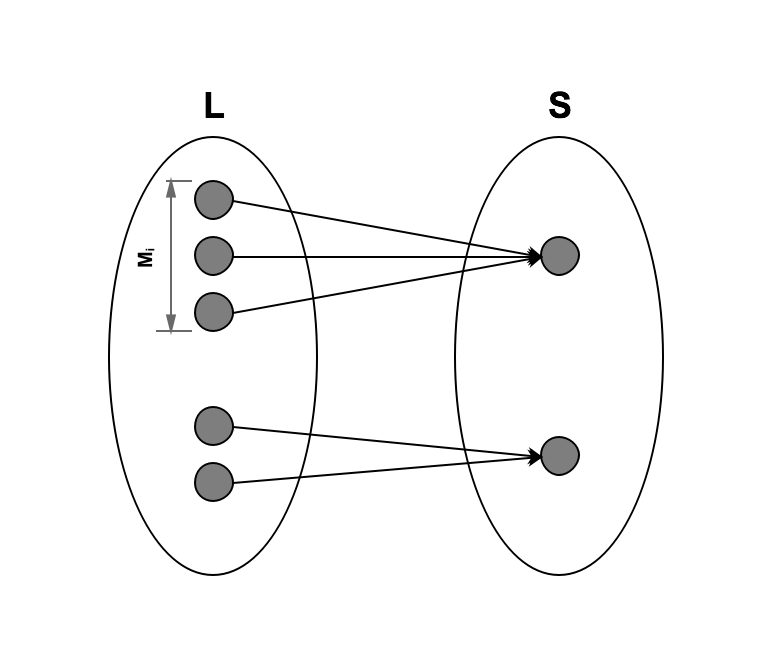
\includegraphics[width=.7\linewidth]{image/falsefork.png}
\caption{ False Fork}
\end{figurehere}
\end{center}

Comme indiqué,$L$ est une collection de tous les comptes forked possibles pour un ensemble de transactions, et $S$ est une collection d'états qui peuvent être atteints avec différents ordres. Selon la définition, \ref{def:fork}, mapping $f: L \rightarrow S$ est un surjectif, et selon la définition \ref{def:falsefork}, ce mapping n'est pas injectif. Ici, nous calculons la probabilité de la fausse fork:

Supposons que $C$ les utilisateurs ont le droit de produire des livres, $M = \vert L \vert$,$N = \vert S \vert$,$M_{i} = \vert L_{i} \vert$, where $L_{i} = \lbrace l \vert f(l) = s_{i}, s_{i} \in S \rbrace$.
La probabilité de fausse fork est la suivante:
\begin{equation}
P_{ff} = \sum_{i=1}^{N}\left ( \frac{M_{i}}{M} \right )^{C} - \frac{1}{M^{C-1}}
\end{equation}

À partir de cette formule, nous pouvons noter que, pour réduire la probabilité de fausse fork, il y a deux manières:
\begin{itemize}
	\item   Établir des relations d'équivalence sur le $L$ d'un ensemble de livre, diviser les classes d'équivalence en eux, et construire moins forked livres.
	\item   Restreindre les utilisateurs qui ont le droit de produire des livres, réduisant ainsi $C$
\end{itemize}

Le premier moyen est la direction importante dans le design du Vite. Nous allons en discuter en détail plus tard. Les deuxièmes moyens ont été acceptés par de nombreux algorithmes. Dans l'algorithme PoW, tout utilisateur a le droit de produire un bloc; et l'algorithme PoS limite la puissance de la production du bloc à ceux qui ont des droits du système; l'algorithme DPoS  \cite{dpos} limite utilisateur sur le droit à  produire le block et être restreint davantage dans un groupe de noeuds d'agent.
	
A présent, Grâce à un algorithme de consensus amélioré, certains projets influents émergent.
Par exemple, Cardano utilise un algorithme de PoS appelé Ouroboros, et la littérature \cite{bernardo2017ouroboros} donne une preuve stricte des caractères liés de l'algorithme; BFT-DPOS algorithme utilisé par EOS\cite{eos}, est une variante de l'algorithme DPoS et améliore la capacité de chargement et déchargement du système en produisant rapidement des blocs; Algorithme de consensus de Qtum \cite{dai2017smart} est aussi un algorithme PoS; L'algorithme de Casper adopté par RChain \cite{rchain} est aussi l'un des algorithmes de PoS..

Il y a aussi d'autres projets qui posent leurs propres propositions pour améliorer l'algorithme de consensus. NEO\cite{neo} utilise un algorithme de BFT, appelé dBFT, et Cosmos\cite{cosmos} utilise un algorithme appelé Tendermint  \cite{tendermint}.

\section{Livre}
\subsection{Aperçu}
Le rôle des livres est de déterminer l'ordre des transactions, et l'ordre des transactions affectera les deux aspects suivants:
\begin{itemize}
	\item \textbf{Cohérence du statut:} Puisque l'état du système n'est pas un TDRC (Types de données répliquées sans conflit) \cite{tdrc}, toutes les transactions ne sont pas échangeables et la séquence d'exécution de la transaction différente peut conduire le système à entrer dans un état différent.
	\item \textbf{Efficacité de Hash:} Dans le livre, la transaction sera empaquetée dans des blocs qui contiennent un hash référencé l'un par rapport à l'autre. L'ordre des transactions affecte la connectivité du hash cité dans les livres. Plus le scope de cet impact soit important, plus le coût de la falsification des transactions est élevé. En effet, toute modification apportée à une transaction doit être reconstruite par hash, qui se réfère directement ou indirectement au bloc de la transaction.
\end{itemize}

Le design du livre a également deux objectifs principaux:

\begin{center}
\begin{figurehere}
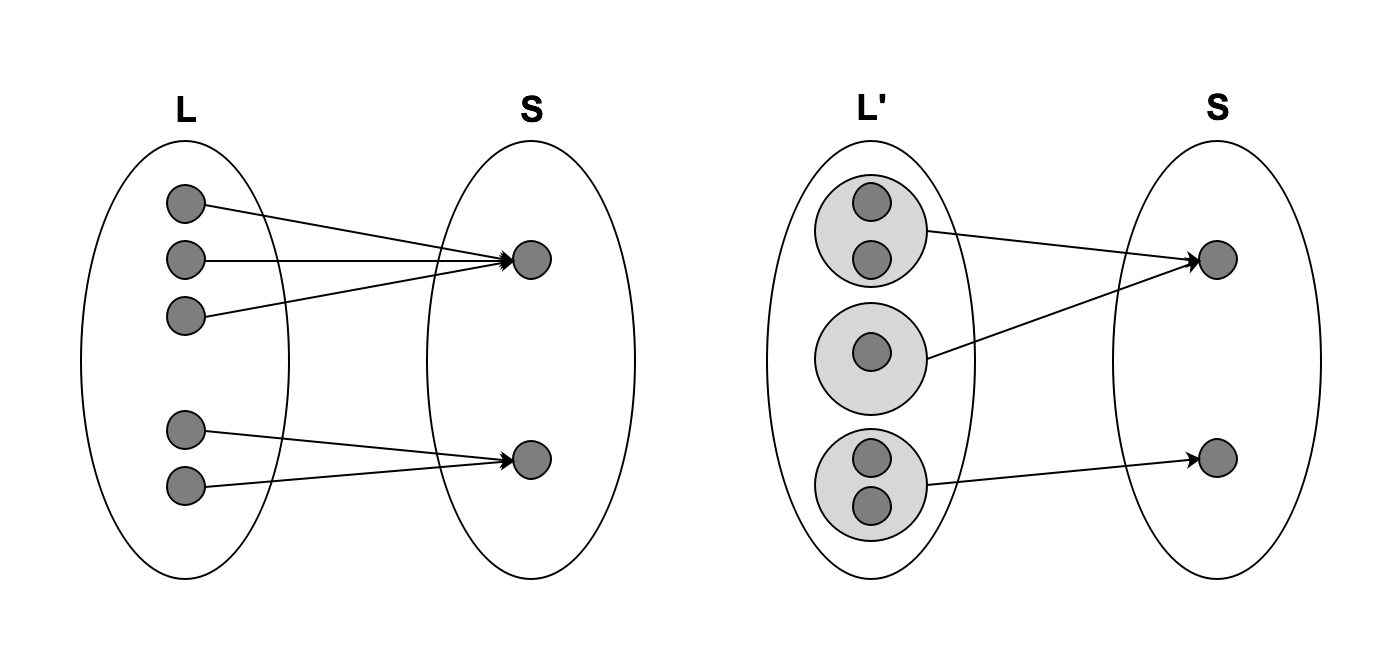
\includegraphics[width=.7\linewidth]{image/ledger-merge.png}
\caption{Ledger merge}
\end{figurehere}
\end{center}

\begin{itemize}
	\item \textbf{Réduire le taux du false fork:} Comme déja discuté dans la section précédente, la réduction du taux de fausse fork peut être obtenue en établissant une classe équivalente et en combinant un groupe de comptes qui amène le système dans le même état dans un seul compte. Comme indiqué ci-dessus, selon la formule de taux de fausse fork, le taux de fausse fork de livre sur la gauche $P_{ff}=\left (  \frac{3}{5} \right )^{C} + \left (  \frac{2}{5} \right )^{C} - \frac{1}{5^{C-1}}$;après la merge de l'espace du livre, le taux de fausse fork du graphique de droite est ${P_{ff}}'=\left (  \frac{2}{3} \right )^{C} + \left (  \frac{1}{3} \right )^{C} - \frac{1}{3^{C-1}}$.On sait que quand $C > 1$,${P_{ff}}' < P_{ff}$. C'est-à-dire que nous devrions minimiser la relation d'ordre partielle entre les transactions et permettre l'échange séquentiel de plus de transactions.
	\item \textbf{Tamper preuve:} lorsqu'une transaction $t$ est modifiée dans le livre $l$,dans les deux sous-livres du livre $l = l_{1} + l_{2}$, le sous livre  $l_{1}$ n'est pas affecté, et les références  du hash dans le sous livre $l_{2}$ doivent être reconstruites pour former un nouveau livre valide ${l}' = l_{1} + {l_{2}}'$. Sous-livre affecté $l_{2} = \Gamma(T_{2}),T_{2} = \lbrace x \vert x \in T, x > t \rbrace $.comme cela, pour augmenter le coût de la falsification des transactions, il est nécessaire de maintenir autant que possible la relation d'ordre partiel entre les transactions afin d'élargir le scope de la falsification $\vert T_{2} \vert$.
\end{itemize}

\begin{center}
\begin{figurehere}
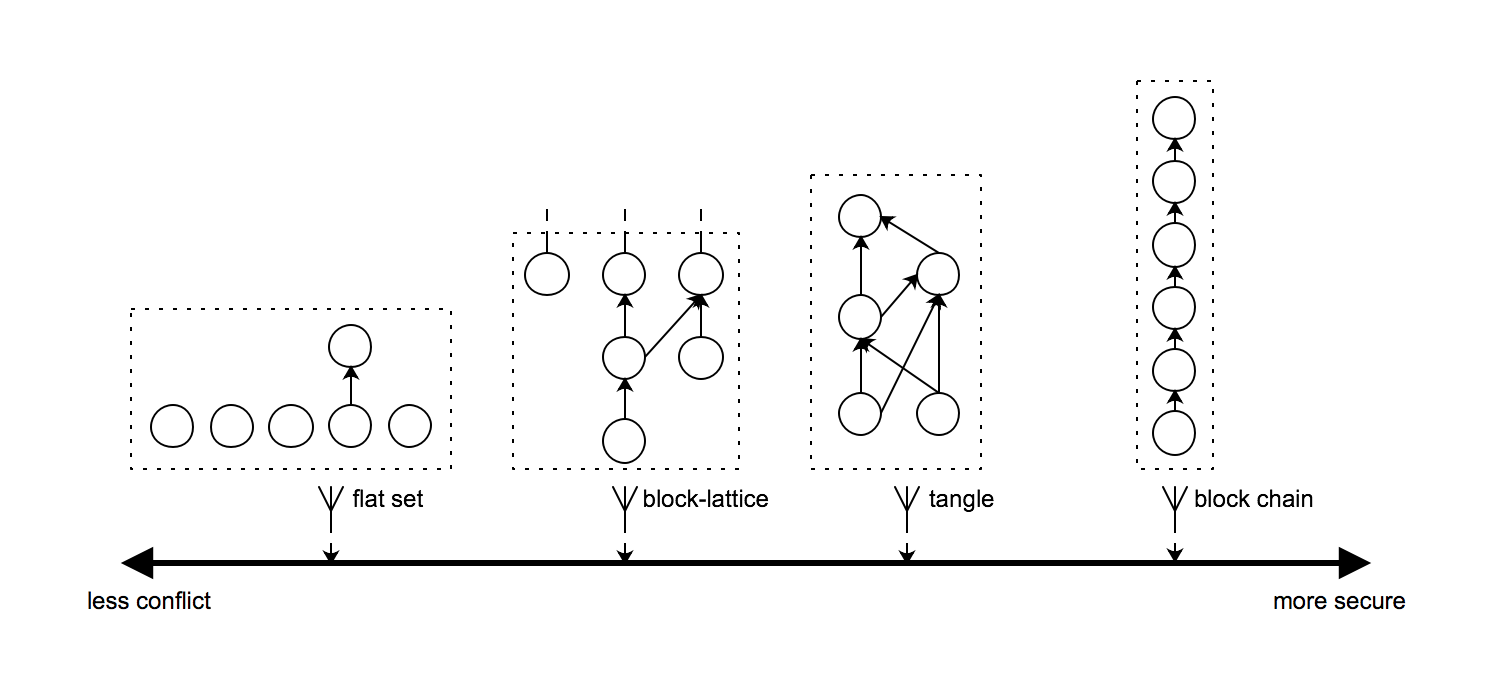
\includegraphics[width=\linewidth]{image/ledger-compare.png}
\caption{Comparaison de la structure du livre}
\end{figurehere}
\end{center}

Evidemment, les deux objectifs ci-dessus sont contradictoires et les arbitrages nécessaires doivent être faits lors de la conception de la structure du compte. Puisque la gestion du compte est un ordre partiel entre les transactions, il s'agit essentiellement d'un ensemble ordonné partiel (poset) \cite{poset}, si représenté par diagramme de Hasse (diagramme de Hasse)\cite{hasse}, c'est un DAG dans la topologie.

L'image ci-dessus compare plusieurs structures de livres communes, et les livres près de la gauche sont maintenus avec moins d'ordre partiel. Le diagramme de Hasse semble plat et il a un taux de fausse fork inférieur; les livres près du côté droit maintiennent plus de relations d'ordre partielles, et le diagramme de Hasse est plus effilé et plus inviolable.

Dans l'image, le côté le plus à gauche est une structure basée sur un ensemble commun dans un système de centralisation sans aucune fonctionnalité d'inviolabilité; le côté le plus à droite est un livre blockchain typique avec les meilleures caractéristiques inviolables; entre les deux, il y a deux livres DAG, le compte de bloc-réseau \cite{nano} utilisé par Nano à gauche; et le côté droit, le livre d'enchevêtrement \cite{iota} est utilisé par l'IOTA. En termes de caractéristiques, le blocklattice maintient moins de relations d'ordre partielles et il est plus adapté à la structure comptable des plates-formes d'applications décentralisées avec hautes performances. En raison de ses mauvaises caractéristiques d'altération, il peut exposer les risques de sécurité, jusqu'à présent, aucun autre projet n'adopte cette structure de livre, sauf Nano.

Afin de poursuivre la haute performance, Vite adopte la structure du livre DAG. En même temps, en introduisant une Snapshot Chain de structure de chaîne supplémentaire et en améliorant l'algorithme de consensus, les failles de la sécurité en réseau de blocs sont correctement résolues, et les deux améliorations seront discutées en détail plus tard.

\subsection{Pré-contrainte}
D'abord, examinons la condition préalable à l'utilisation de cette structure de livre pour le modèle de machine d'état. Cette structure est essentiellement une combinaison de la machine d'état entière en tant qu'ensemble de machines d'état indépendantes, chaque compte correspondant à une machine d'état indépendante, et chaque transaction n'affecte que l'état d'un seul compte. Dans le livre, toutes les transactions sont regroupées dans des comptes et organisées en une chaîne de transactions dans le même compte. Par conséquent, nous avons les restrictions suivantes sur l'état S et la transaction T dans Vite:

\begin{definition}[Contrainte de liberté d'un seul degré]
l'état du système $s \in S$,est le vecteur $s=(s_{1}, s_{2},...,s_{n})$ formé par l'état $s_{i}$ de chaque compte. Pour $\forall t_{i} \in T$,après effectuer la transaction $t_{i}$, l'état du système est transféré comme suit: $({s_{1}}',..., {s_{i}}',...,{s_{n}}') = \sigma(t_{i}, (s_{1},..., s_{i},...,s_{n}))$,il nécessite de répondre à la condition:${s_{j}}'=s_{j} , j \neq i$.Cette contrainte est appelée contrainte de liberté d'un seul degré pour une transaction.
\end{definition}

Intuitivement, une transaction avec la liberté d'un seul degré changera seulement l'état d'un compte sans affecter le statut d'autres comptes dans le système. Dans l'espace multidimensionnel où se trouve le vecteur d'espace d'état, une transaction est exécutée et l'état du système ne se meut que au long de la direction parallèle à un axe de coordonnées. Veuillez noter que cette définition est plus stricte que la définition de transaction dans Bitcoin, Ethereum et d'autres modèles. Une transaction dans Bitcoin changera l'état des deux comptes de l'expéditeur et du destinataire; l'Ethereum peut changer l'état de plus de deux comptes via un appel de message.

Sous cette contrainte, la relation entre les transactions peut être simplifiée. Toute transaction est orthogonale ou parallèle. Cela fournit des conditions pour regrouper les transactions selon les comptes. Voici un exemple à expliquer:

\begin{center}
\begin{figurehere}
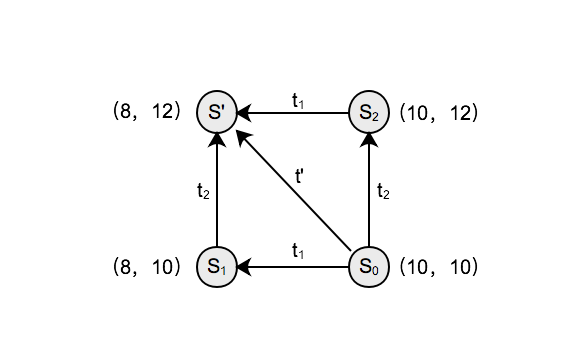
\includegraphics[width=.8\linewidth]{image/tx-deg-of-free.png}
\caption{Single degree of freedom trading and intermediate state}
\end{figurehere}
\end{center}

Comme montré dans la figure ci-dessus, supposons qu'Alice et Bob aient respectivement 10 USD. L'état initial du système est $s_{0} = (10, 10)$. Quand Alice veut transférer 2 USD à Bob, dans le modèle de Bitcoin et Ethereum, une transaction${t}'$,peut conduire le système directement à l'état final:$s_{0} \overset{{t}'}{\rightarrow}{s}'$.

Dans la définition de Vite, la transaction ${t}'$ a également modifié le statut de deux comptes d'Alice et de Bob, ce qui n'était pas conforme au principe de de liberté d'un seul degré. Par conséquent, la transaction doit être scindée en deux transactions:

1) Une transaction $t_{1}$ représentant le transfert de 2 USD par Alice

2) Une transaction $t_{2}$ représente la réception de 2 USD par Bob 

De cette manière, de l'état initial à l'état final ${s}'$ il pourrait y avoir deux chemins différents $s_{0} \overset{t_{1}}{\rightarrow} s_{1} \overset{t_{2}}{\rightarrow} {s}'$ et $s_{0} \overset{t_{2}}{\rightarrow} s_{2} \overset{t_{1}}{\rightarrow} {s}'$. Ces deux chemins sont respectivement passés à travers l'état intermédiaire $s_{1}$ et $s_{2}$, et ces deux états intermédiaires sont le mapping de l'état final ${s}'$ dans la dimension de ces deux comptes.En d'autres termes, si vous voudriez savoir uniquement de l'état de l'un des comptes, vous devez uniquement exécuter toutes les transactions qui correspondent au compte et ne pas avoir à effectuer les transactions des autres comptes.

Ensuite, nous allons définir comment diviser les transactions dans Ethereum en transactions à un seul degré de liberté requises par Vite:
\begin{definition}[Décomposition de transaction]
Division d'une transaction avec le degré de liberté supérieur à 1 en un ensemble de transactions avec liberté en un seul degré, dénommé Décomposition des transactions. Une transaction de transfert peut être divisée en une transaction d'envoi et une transaction de réception; une transaction d'appel de contrat peut être divisée en une transaction de demande de contrat et une transaction de réponse de contrat; un appel de message dans chaque contrat peut être divisé en une transaction de demande de contrat et une transaction de réponse contractuelle.
\end{definition}

Donc, il y aurait deux types différents de transactions dans les livres. Ils sont appelés "paires de négoce":
\begin{definition}[paires de négoce]
une transaction d'envoi ou une transaction de demande de contrat, collectivement appelée "transaction de demande"; une transaction de réception ou une transaction de réponse de contrat, collectivement appelée "transaction de réponse". Une transaction de requête et une transaction de réponse correspondante sont appelées paires de transactions. Le compte pour initier la demande de transaction $t$  est enregistré comme $A(t)$; la transaction de réponse correspondante est enregistrée comme: $\widetilde{t}$, le compte correspondant à la transaction est enregistré comme  $A(\widetilde{t})$.
\end{definition}

Basé sur la définition ci-dessus, nous pouvons conclure la relation possible entre deux transactions de Vite:
\begin{definition}[Relation de transaction]
Il peut exister pour les relations suivantes pour deux transactions $t_{1}$ and $t_{2}$:

\textbf{Orthogonalité}:Si $A(t_{1}) \neq A(t_{2})$,les deux transactions sont orthogonales, enregistrées  comme: $t_{1} \perp t_{2}$;

\textbf{Parallèle}:Si $A(t_{1}) = A(t_{2})$,les deux transactions sont parallèles, enregistrées comme $t_{1} \parallel t_{2}$;

\textbf{Causalité}:Si $t_{2} = \widetilde{t_{1}}$,alors les deux transactions sont raisonnables, enregistrées comme $t_{1} \rhd t_{2}$, or $t_{2} \lhd t_{1}$.
\end{definition}

\subsection{Définition du Livre}
Pour définir un livre, c'est définir un poset. Tout d'abord, définissons la relation d'ordre partielle entre les transactions dans Vite:
\begin{definition}[Ordre partiel des transactions]
Nous utilisons une relation dualiste $<$ pour représenter la relation d'ordre partiel de deux transactions:
Une transaction de réponse doit suivre une transaction de demande correspondante:$t_{1} < t_{2} \Leftrightarrow t_{1} \rhd t_{2}$;

Toutes les transactions sur un compte doivent être strictement et globalement ordonnées:$\forall t_{1} \parallel t_{2}$, la condition doit être satisfait :$t_{1} < t_{2}$,ou $t_{2} < t_{1}$.
\end{definition}

Dû à la relation de commande partielle établie sur l'ensemble de transaction $T$ répondent aux caractéristiques:
\begin{itemize}
	\item Irréflexive: $\forall t \in T$,il n'y a pas $t < t$;
	\item Transitif:$\forall t_{1},t_{2},t_{3} \in T$, Si $t_{1}<t_{2},t_{2}<t_{3}$, puis $t_{1}<t_{3}$;
	\item Asymétrique:$\forall t_{1},t_{2} \in T$, if $t_{1}<t_{2}$, alors ça n'existe pas $t_{2}<t_{1}$
\end{itemize}

De cette façon, nous pouvons définir le compte Vite dans un ensemble d'ordre partiel strict:

\begin{definition}[Livre de Vite]
Vite Ledger est un poset restreint composé de l'ensemble de $T$ de la transaction donnée, et du poset partiel $<$ 
\end{definition}

\begin{center}
\begin{figurehere}
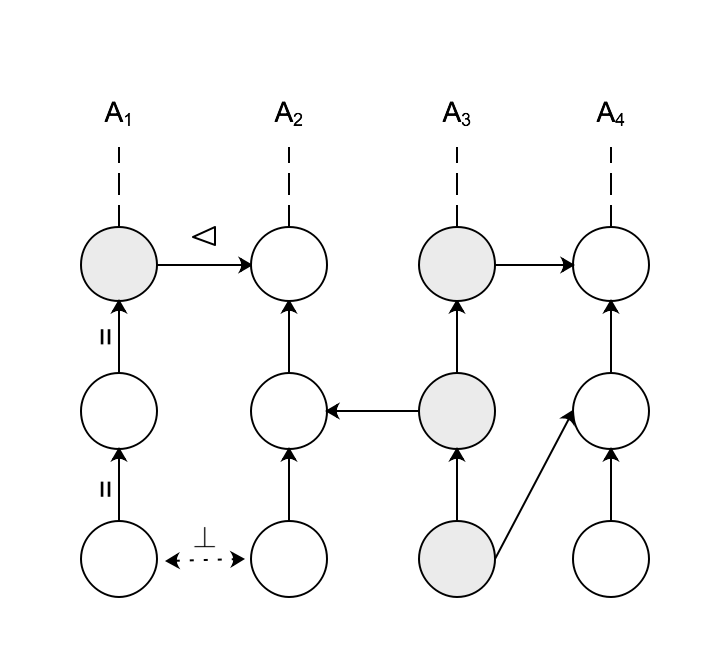
\includegraphics[width=.7\linewidth]{image/ledger.png}
\caption{La relation entre le livre et la transaction à Vite}
\end{figurehere}
\end{center}

Un poset strict peut correspondre à une structure DAG. Comme montré dans la figure ci-dessus, les cercles représentent les transactions et les flèches indiquent les dépendances entre les transactions. $a \rightarrow b$ indique que $a$ dépend à $b$.

Le livre du Vite défini ci-dessus est structurellement similaire à un treillis-bloc. Les transactions sont divisées en transactions de requête et de réponse, chacune correspondant à un bloc distinct, chaque compte Ai correspond à une chaîne, une paire de transactions et une transaction de réponse référençant le hash de sa transaction de requête correspondante.

\section{Chaîne instantanée}
\subsection{Confirmation de transaction}
Lorsque le compte est forked, le résultat du consensus peut osciller entre deux livres forked. Par exemple, sur la base d'une structure blockchain, si un nœud reçoit une chaîne forked plus longue, la nouvelle fork sera sélectionnée comme résultat consensuel et la fork d'origine sera abandonnée et la transaction sur la fork d'origine sera annulée. Dans un tel système, l'annulation d'une transaction est un événement très grave, ce qui entraînera une double dépense. Imaginez juste qu'une entreprise reçoit un paiement, fournit des biens ou des services, et après que le paiement est retiré, le commerçant peut rencontrer des pertes. Par conséquent, lorsqu'un utilisateur reçoit une transaction de paiement, il doit attendre que le système "confirme" la transaction pour s'assurer que la probabilité de reculer est suffisamment faible.

\begin{definition}[Confirmation de Transaction]
lorsque la probabilité d'annulation d'une transaction est inférieure à un seuil donné $\epsilon$, la transaction est considérée comme confirmée.
$P_{r}(t) < \epsilon \Leftrightarrow t \text{ is } \boldsymbol{confirmed}$.
\end{definition}


La confirmation des transactions est un concept très déroutant, parce que la reconnaissance d'une transaction dépend en fait du niveau de confiance implicite de $1-\epsilon$. Un commerçant vendant des diamants et un vendeur de café ont subi des pertes différentes lorsqu'ils ont été attaqués par une double dépense. En conséquence, le premier doit définir $\epsilon$ plus petit sur la transaction. C'est aussi l'essence du nombre de confirmations dans Bitcoin. Dans Bitcoin, le numéro de confirmation indique la profondeur d'une transaction dans la chaîne de blocs. Plus le nombre de confirmations est élevé, plus la probabilité d'annulation de la transaction est faible \ cite {nakamoto2008bitcoin}. Par conséquent, les commerçants peuvent définir indirectement le niveau de confiance de la confirmation en définissant le nombre de numéros de confirmation en attente.


La probabilité d'annulation d'une transaction diminue avec le temps dû à la relation de référence de hash dans la structure du compte. Comme mentionné ci-dessus, lorsque la conception du livre a de meilleures caractéristiques d'altération, l'annulation d'une transaction doit reconstruire tous les blocs suivants de l'échange dans le bloc. Comme de nouvelles transactions sont constamment ajoutées aux livres, il y a de plus en plus de nœuds successifs dans une transaction, donc la probabilité d'être trafiqué diminuera. 

Dans la structure block-treillis, comme la transaction est groupée par compte, une transaction ne sera attachée qu'à la fin de la chaîne de compte de son propre compte, et la transaction générée par la plupart des autres comptes ne deviendra pas automatiquement un nœud successeur de la transaction. Par conséquent, il est nécessaire de concevoir un algorithme de consensus raisonnablement pour éviter les dangers cachés de double dépense.

Nano adopte un algorithme de consensus basé sur le vote, \cite{nano}, la transaction est signée par un ensemble de nœuds représentatifs sélectionnés par un groupe d'utilisateurs. Chaque noeud représentatif a un poids. Lorsque la signature d'une transaction a assez de poids, on croit que la transaction est confirmée. Il y a des problèmes suivants dans cet algorithme:

Premièrement, si la confirmation avec le degré de confiance plus élevé est nécessaire, le seuil du poids de vote doit être augmenté. S'il n'y a pas assez de nœuds représentatifs en ligne, la vitesse d'intersection ne peut pas être garantie, et il est possible qu'un utilisateur ne recueille jamais le nombre de tickets nécessaire pour confirmer un échange;

Deuxièmement, la probabilité que les transactions soient annulées ne diminue pas au fils du temps. En effet, à tout moment, le coût du renversement d'un vote historique est le même.

Enfin, les résultats de vote historiques ne sont pas conservés dans le livre et sont stockés uniquement dans le stockage local des noeuds. Lorsqu'un nœud obtient son compte auprès d'autres nœuds, il n'existe aucun moyen de quantifier de façon fiable la probabilité d'annulation d'une transaction historique.

En effet, le mécanisme de vote est une solution de centralisation partielle. Nous pouvons considérer les résultats du vote comme un instantané de l'état des livres. Cet instantané sera distribué dans le stockage local de chaque noeud du réseau. Afin d'avoir la même capacité inviolable avec la chaîne de blocs, nous pouvons également organiser ces instantanés en structures de chaîne, qui est l'un des noyaux de la conception de Vite - la chaîne de clichés \cite{snapshotchain}.

\subsection{Définition de chaîne instantanée}
La chaîne instantanée est la structure de stockage la plus importante de Vite. Sa fonction principale est de maintenir le consensus de Vite livre. D'abord, nous donnons la définition de la chaîne instantanés: 
\begin{definition}[Bloc d'instantanés et chaîne d'instantanés]
un bloc d'instantané qui stocke un état instantané d'un Vite livre, y compris le solde du compte, la racine Merkle de l'état du contrat et le hash du dernier bloc dans chaque chaîne de comptes. La chaîne instantanés est une structure en chaîne composée de blocs instantanés et le bloc d'instantanés suivant fait référence au hash du bloc instantanés précédent.
\end{definition}

L'état d'un compte d'utilisateur contient le solde et le hash du dernier bloc de la chaîne de compte; en plus des deux champs ci-dessus, l'état d'un compte de contrat contient le hash racine de Merkle, la structure de l'état d'un compte est la suivante:

\begin{verbatim}
  struct AccountState {
    // account balance
    map<uint32, uint256> balances;
    // Merkle root of the contract state
    optional uint256 storageRoot;
    // hash of the last transaction
    // of the account chain
    uint256 lastTransaction;
  }
\end{verbatim}

La structure du bloc instantané est définie comme le suivant:
\begin{verbatim}
  struct SnapshotBlock {
    // hash of the previous block   
    uint256 prevHash;
    // snapshot information
    map<address, AccountState> snapshot;
    // signature
    uint256 signature;
  }
\end{verbatim}

Afin de prendre en charge plusieurs jetons en même temps, la structure d'enregistrement des informations de solde dans l'état de compte de Vite n'est pas une \texttt{uint256}, mais un mapping a partir de token ID à la balance.

Le premier block instantané dans la chaîne d'instantanés est appelé «instantané de genèse», qui enregistre des instances du bloc de genèse dans le compte.

\begin{center}
\begin{figurehere}
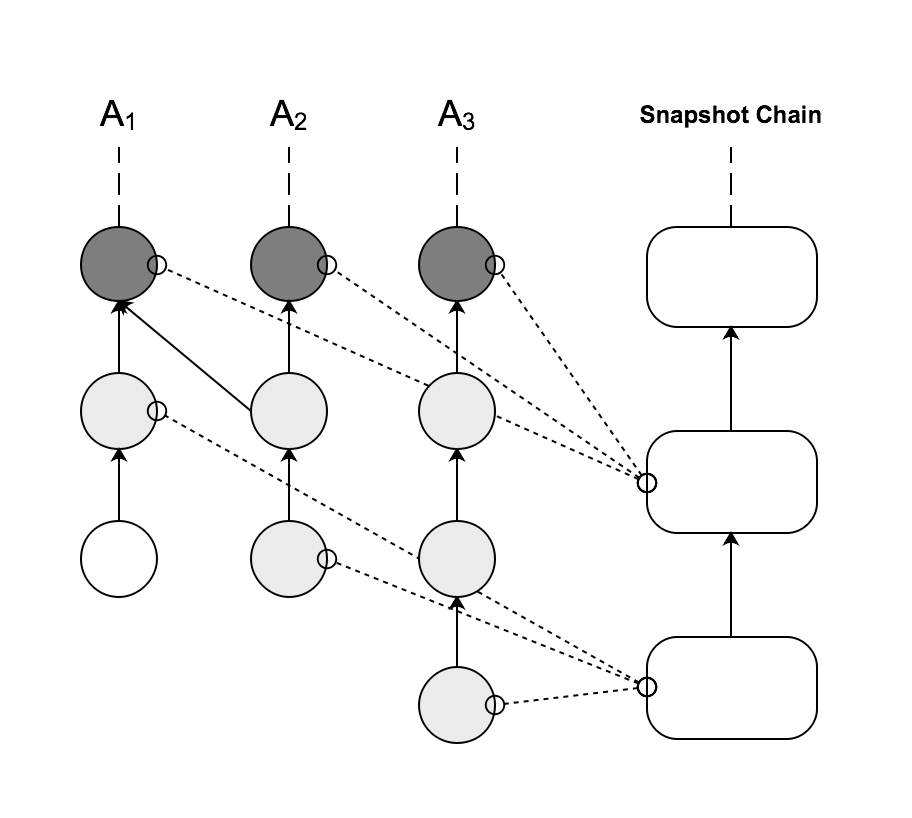
\includegraphics[width=.7\linewidth]{image/snapshotchain.png}
\caption{snapshot chain}
\end{figurehere}
\end{center}

Étant donné que chaque bloc instantané dans la chaîne instantanée correspond à la seule fork du livre Vite, il est possible de déterminer le résultat consensuel du livre Vite par le bloc instantanés lorsque le bloc instantanés ne passe pas dans le bloc d'instantané.

\subsection{Chaîne instantanée et confirmation de transaction}

Après l'introduction de la chaîne instantanée, les défauts de sécurité naturels de la structure en treillis ont été corrigés. Si un attaquant veut générer une transaction de double dépense, en plus de reconstruire la référence de hash dans le livre Vite, il doit également être reconstruit dans la chaîne instantanée pour tous les blocs après le premier bloc instantané de la transaction, et doit produire une chaîne instantanée plus longue. De cette façon, le coût de l'attaque sera considérablement augmenté.

Dans Vite, le mécanisme de confirmation des transactions est similaire à Bitcoin, qui est défini comme suit:

\begin{definition}[Confirmation de Transaction dans Vite]
Dans Vite, si une transaction est une instance par la chaîne instantanée, la transaction est confirmée, la profondeur du bloc instantanée dans le premier instance, est appelée le numéro de confirmation de la transaction.
\end{definition}

Selon cette définition, le nombre de transactions confirmées augmentera de 1 lorsque la chaîne instantanée augmentera, et la probabilité de l'attaque de double dépense diminuera avec l'augmentation de la chaîne d'instantanée. De cette manière, les utilisateurs peuvent personnaliser le numéro de confirmation requis en attendant différents numéros de confirmation selon le scénario spécifique.

La chaîne instantanée elle-même repose sur un algorithme de consensus. Si la chaîne instantanée est forkée, le fork \ textbf {longest} est choisi comme fork valide. Lorsque la chaîne instantanée est passée à une nouvelle branche, les informations instantanées d'origine seront annulées, ce qui signifie que le consensus original sur le livre a été renversé et remplacé par le nouveau consensus. Par conséquent, la chaîne instantanée est la première pierre de la sécurité du système entier, et doit être traitée sérieusement.

\subsection{Compressed storage}
Car tous les états de compte doivent être enregistrés dans chaque bloc instantané dans la chaîne instantanée, l'espace de stockage doit être très grand, la compression vers les chaînes instantanées est nécessaire.

\begin{center}
\begin{figurehere}
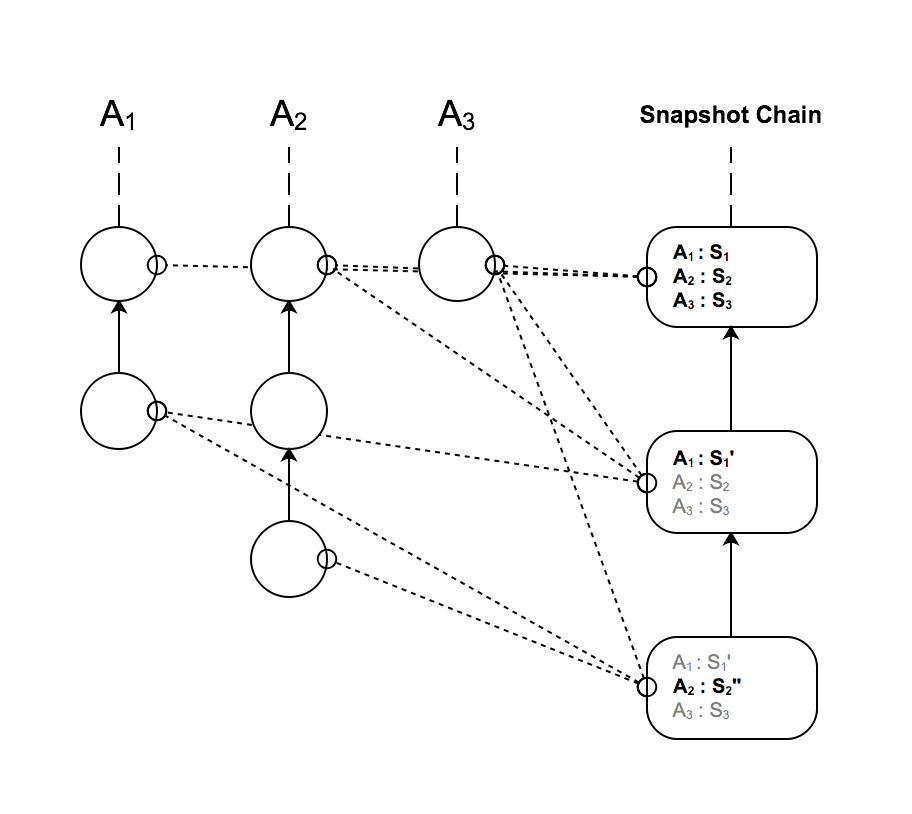
\includegraphics[width=.7\linewidth]{image/compact-snapshot.png}
\caption{Instantané avant compression}
\end{figurehere}
\end{center}

L'approche de base de la compression de l'espace de stockage de la chaîne instantanée consiste à utiliser le stockage incrémentiel: un bloc instantané stocke uniquement les données modifiées par rapport au bloc instantané précédent. S'il n'y a pas de transaction pour un compte entre les deux instantanés, le dernier bloc instantané n'enregistrera pas les données du compte.

Pour récupérer des informations instantanés, vous pouvez parcourir le bloc instantané du début à la fin et couvrir les données de chaque bloc instantanés en fonction des données en cours.

\begin{center}
\begin{figurehere}
\centering
\tikzstyle{block} = [draw, fill=blue!20, rectangle, 
    minimum height=3em, minimum width=6em]
\tikzstyle{sum} = [draw, fill=blue!20, circle, node distance=1cm]
\tikzstyle{input} = [coordinate]
\tikzstyle{output} = [coordinate]
\tikzstyle{pinstyle} = [pin edge={to-,thin,black}]

\begin{tikzpicture}[
    auto, 
    node distance=2cm,
    >=latex',
    font=\bfseries\footnotesize\sffamily,
    snapshot/.style={
		scale=0.7,
		rectangle,
		rounded corners,
		draw=black, 
		text centered,
%		text width=5cm,
		minimum height=12mm,
		fill=white
	},
	label/.style={
		scale=0.7
	}
  ]
    % We start by placing the blocks

  \node [snapshot] (snapshot2) 
 {%
 \begin{tabular}{l}
  \textbf{Snapshot\#2}\\
  $A_{1}: {s_{1}}'$\\
  \\
  \\
 \end{tabular}
 };
 
  \node [snapshot, xshift=-3.5cm] (snapshot1) 
 {%
 \begin{tabular}{l}
  \textbf{Snapshot\#1}\\
  $A_{1}: s_{1}$\\
  $A_{2}: s_{2}$\\
  $A_{3}: s_{3}$
 \end{tabular}
 };
 
 
  \node [snapshot, xshift=3.5cm] (snapshot3) 
 {%
 \begin{tabular}{l}
  \textbf{Snapshot\#3}\\
  \\
  $A_{2}: {s_{2}}''$\\
  \\
 \end{tabular}
 };
 
 \draw [draw,->] (snapshot2) -- (snapshot1);
 \draw [draw,->] (snapshot3) -- (snapshot2);

\end{tikzpicture}

\caption{Instantané après compression}
\label{fig:compact-snapshot}
\end{figurehere}
\end{center}

Que le status final de chaque instantané d'un compte est sauvegardé lors qu'il est capturé, l'état intermédiaire ne sera pas pris en compte, de sorte qu'une seule copie des données instantanés sera sauvegardée, quel que soit le nombre de transactions générées par un compte entre deux instantanés. Par conséquent, un bloc instantané prend jusqu'à $S * A$ octets au maximum. Parmi eux, $S = \text{sizeof}(s_{i})$, est le nombre d'octets occupés pour chaque état de compte, et $A$ est le nombre total de comptes sur le système. Si le taux moyen des comptes actifs par rapport au total est $a$, le taux de compression est de $1-a$.

\section{Consensus}
\subsection{Goal of Design}
Lors concevoir un protocole de consensus, nous devons prendre en compte les facteurs suivants:
\begin{itemize}
	\item \textbf{Performance}.L'objectif principal de Vite est rapide. Pour garantir un chargement et déchargement élevé et des performances avec faible retard du système, nous devons adopter un algorithme de consensus avec une vitesse de convergence plus élevée.
	\item \textbf{Scalability}.Vite est une plate-forme publique et ouverte à toutes les applications décentralisées, donc l'évolutivité est également un facteur important.
	\item \textbf{Security}.Le principe de conception de Vite ne poursuit pas la sécurité extrême, cependant, il doit toujours assurer une ligne de base de sécurité suffisante et se prémunir efficacement contre toutes sortes d'attaques.
\end{itemize}

Comparé à certains algorithmes de consensus existants, la sécurité de PoW est meilleure, et un consensus peut être atteint si la puissance de calcul des nœuds malveillants est inférieure à 50\%. Cependant, la vitesse d'intersection de PoW est lente et ne peut pas répondre aux exigences de performance; Le PoS et ses variantes d'algorithmes éliminent les étapes permettant de résoudre les problèmes mathématiques, d'améliorer la vitesse d'intersection et le coût d'attaque unique, et de réduire la consommation d'énergie. Mais l'évolutivité du PoS est encore faible, et le problème "Nothing at Stake" \cite{problems} est difficile à résoudre; Les algorithmes BFT ont de meilleures performances en termes de sécurité et de performances, mais leur évolutivité est un problème, généralement plus adapté à une chaîne privée ou à une chaîne de consortium; l'algorithme DPoS \cite{dpos} réduit efficacement la probabilité de fausse fork en limitant les permissions de génération de blocs. Les performances et l'évolutivité sont bonnes. En conséquence, DPoS a un léger sacrifice de sécurité, et le nombre de nœuds malveillants ne doit pas dépasser 1/3 \cite{dpos2}.

Généralement, l'algorithme DPoS présente des avantages évidents en termes de performances et d'évolutivité. Par conséquent, nous choisissons DPoS comme la base du protocole de consensus Vite et nous l'étendons correctement sur la base de celui-ci. Grâce au protocole de consensus hiérarchique délégué et au modèle asynchrone, la performance globale de la plateforme peut être encore améliorée.

\subsection{Hierarchical Consensus}
The consensus protocol of Vite is HDPoS (Preuve de participation déléguée et hiérarchique). L'idée de base est de décomposer la fonction de consensus $\Phi$ (la décomposition fonctionnelle):
\begin{equation}
\begin{split}
\Phi(l_1,l_2,\dots,l_n) = \Psi(\Lambda_1(l_1,l_2,\dots,l_n), \\
\Lambda_2(l_1,l_2,\dots,l_n),\dots \\
\Lambda_m(l_1,l_2,\dots,l_n))
\end{split}
\end{equation}

$\Lambda_i: 2^L \rightarrow L$,est appelé comme fonction de consensus local, le résultat renvoyé est appelé le consensus local; $\Psi: 2^L \rightarrow L$, connu sous le nom de la fonction de consensus globale, il sélectionne un résultat unique d'un groupe de candidat dans un consensus comme le résultat final consensuel.

Après cette séparation, le consensus de l'ensemble du système est devenu deux processus indépendants:
\begin{labeling}{alligator}
\item [Consensus local] générer les blocs correspondant aux transactions de requête et de transaction de réponse dans le compte d'utilisateur ou le compte de contrat, et écrire dans les ledgers.
\item [Global consensus] instantanés les données dans le livre et génère des blocs instantanés. Si le registre est forked, choisissez-en un.
\end{labeling}

\subsection{Right of Block Generation and Consensus Group}
Ensuite, qui a le droit de générer le bloc de transaction dans le bloc-notes et le bloc instantané dans la chaîneinstantanée? Quel algorithme de consensus est adopté pour parvenir à un consensus?
Comme la structure de livre de Vite est organisée en plusieurs chaînes de compte selon différents comptes, nous pouvons définir facilement le droit de production des blocs dans le livre en fonction de la dimension du compte, et le droit de production du bloc instantané appartient à à un seul groupe d'utilisateurs. De cette manière, nous pouvons mettre un certain nombre de chaînes de comptes ou de chaînes instantanée dans un groupe de consensus, et dans le groupe de consensus, nous pouvons utiliser une manière unifiée pour produire le bloc et atteindre un consensus.

\begin{definition}[Consensus Group]
Consensus group is a tuple $(L, U, \Phi, P)$, describing the consensus mechanism of a portion of the account or snapshot chain.,$L \in A \vert \{ A_s \}$,  represents one or a number of account chains, or snapshot chains of the consensus group in the ledger; $U$ represents the user with the block production right on the chain specified by the $L$; $\Phi$ specifies the consensus algorithm of the consensus group; and $P$ specifies the parameters of the consensus algorithm.

\end{definition}

D'apès cette définition, les utilisateurs peuvent définir des groupes de consensus de manière flexible et sélectionner différents paramètres de consensus sur leurs besoins. Ensuite, nous allons élaborer sur les différents groupes de consensus.

\subsubsection{Groupe de consensus instantané}
Le groupe de consensus des chaînes instantanées est appelé groupe de consensus instantané, qui est le groupe de consensus le plus important de Vite. L'algorithme de consensus $\Phi$ du groupe consensus instantané adopte l'algorithme DPoS et correspond à $\Psi$ dans le modèle hiérarchique. Le nombre d'agents et l'intervalle de génération du bloc sont spécifiés par le paramètre $P$.

For example, we can specify snapshot consensus groups with 25 proxy nodes to produce snapshot blocks at intervals of 1 second. This ensures that the transaction is confirmed to be fast enough. Achieving 10 times transaction confirmation need to wait 10 seconds in maximum.

\subsubsection{Private Consensus Group}
Par exemple, nous pouvons spécifier des groupes consensus instantanés avec 25 noeuds proxy pour produire des blocs instantanés à intervalles de 1 seconde. Cela garantit que la transaction est confirmée pour être assez rapide. Obtenir 10 fois la confirmation de la transaction doit attendre 10 secondes au maximum. 

Le plus grand avantage du groupe de consensus privé est de réduire la probabilité de fork. Car un seul utilisateur a le droit de produire des blocs, la seule possibilité de fork est que l'utilisateur initie une double attaque personnelle ou une erreur de programme.

L'inconvénient du groupe de consensus privé est que les nœuds utilisateur doivent être en ligne avant de pouvoir emballer la transaction. Ce n'est pas très convenable pour le compte du contrat. Une fois que le nœud du propriétaire a échoué, aucun autre nœud ne peut remplacer la transaction de réponse qu'il produit, ce qui équivaut à réduire la disponibilité du service dApp.


\subsubsection{Delegate Consensus Group}
Dans le groupe de consensus délégué, au lieu du compte d'utilisateur, un ensemble de noeuds proxy désignés est utilisé pour conditionner la transaction via l'algorithme DPoS. A la fois les comptes d'utilisateur et les comptes contractuels peuvent être ajoutés au groupe de consensus. Les utilisateurs peuvent définir un ensemble de nœuds d'agent distincts et établir un nouveau groupe de consensus. Il existe également un groupe de consensus par défaut dans Vite pour aider à regrouper les transactions pour tous les autres comptes qui n'ont pas établi individuellement leur groupe de consensus délégués, également connu sous le nom de \textbf {groupe de consensus public}.

Le groupe de consensus délégué convient à la plupart des comptes de contrats, car la plupart des transactions dans le contrat du compte sont des transactions de réponse de contrat, pour lesquelles une disponibilité plus élevée et des délais plus courts sont nécessaires au lieu des transactions recevables dans le compte utilisateur.

\subsection{La priorité du consensus}\label{sec:consensus-prio}
Dans le protocole de Vite, la priorité du consensus global est supérieure à celle du consensus local. Lorsque le consensus local est forked, le résultat de la sélection du consensus mondial prévaudra. En d'autres termes, une fois que le consensus global a sélectionné un fork du consensus local comme le résultat final, même un fork plus longue d'une certaine chaîne de compte dans les comptes futurs se produit, elle ne provoquera pas le retour des résultats du consensus global.

Nous devons faire plus attention à ce problème lors de la mise en œuvre du protocole cross-chain. Étant donné qu'une chaîne cible peut revenir en arrière, la chaîne de comptes correspondante du contrat de relais qui mappe la chaîne doit également être annulée en conséquence. A ce moment, si le consensus local de la chaîne de relais a été adopté par le consensus global, il est impossible de terminer le rollback, ce qui peut rendre incohérentes les données entre le contrat de relais et la chaîne cible.

La manière d'éviter ce problème est de définir un paramètre \textit{delay}  dans le paramètre de groupe de consensus $P$, qui spécifie le groupe de consensus instantané pour prendre un instantané seulement le consensus local est terminé après les blocs \textit{delay}. Cela réduira considérablement la probabilité d'incohérence des contrats de relais, mais elle ne peut pas être complètement évitée. Dans la logique de code des contrats de relais, il est également nécessaire de traiter séparément la restauration de la chaîne cible.

\subsection{Modèle asynchrone}
Afin d'améliorer davantage le chargement et déchargement du système, nous devons supporter un modèle asynchrone plus parfait sur le mécanisme du consensus.

Le cycle de vie d'une transaction comprend l'initiation de la transaction, la rédaction de la transaction et la confirmation de la transaction. Afin d'améliorer les performances du système, nous devons concevoir ces trois étapes en mode asynchrone. En effet, à moments différents, le nombre de transactions initiées par les utilisateurs est différent, la rapidité de l'écriture des transactions et la confirmation des transactions traitées par le système sont fixées de manière relative. Le mode asynchrone aide à aplatir les pics et les creux, donc améliore le chargement et déchargement global du système.
 

Le modèle asynchrone du Bitcoin et de l'Ethereum est simple: la transaction initiée par tous les utilisateurs est placée dans un pool non confirmé. Lorsque le mineur l'empaquette dans un bloc, la transaction est écrite et confirmée en même temps. Lorsque la chaîne de blocs continue à croître, la transaction atteint finalement le niveau de confiance de confirmation prédéfini.

Il y a deux problèmes dans ce modèle asynchrone:
\begin{itemize}
	\item	Les transactions ne sont pas insistant aux livres dans un état non confirmé. Les transactions non reconnues sont instables et ne font l'objet d'aucun consensus. Elles ne peuvent empêcher répéter l'envoi de transactions.
	\item	Il n'y a pas de mécanisme asynchrone pour l'écriture et la confirmation des transactions. Les transactions ne sont écrites que lorsqu'elles sont confirmées, et la vitesse d'écriture est limitée par la vitesse de confirmation.
\end{itemize}

Le protocole de Vite établit un modèle asynchrone amélioré: d'abord, la transaction est divisée en une paire de transactions basée sur un modèle "requête-réponse",qu'il s'agisse d'un transfert ou d'un contrat, et la transaction est lancée avec succès est écrit dans le livre. De plus, l'écriture et la confirmation d'une transaction sont également asynchrones. Les transactions peuvent d'abord être écrites dans le compte DAG de Vite et ne seront pas bloquées par le processus de confirmation. La confirmation de la transaction est effectuée via la chaîne d'instantané, et l'action d'instantané est également asynchrone.

C'est un modèle producteur-consommateur typique. Dans le cycle de vie de la transaction, quel que soit le changement de taux de production en amont, l'aval peut traiter la transaction à un rythme constant, de manière à utiliser pleinement les ressources de la plate-forme et améliorer le débit du système.

\section{Machine Virtuelle}
\subsection{Compatibilité EVM}
A présent, il existe de nombreux développeurs dans le domaine Ethereum, et de nombreux contrats intelligents sont appliqués sur la base de Solidity et EVM. Par conséquent, nous avons décidé de fournir une compatibilité EVM sur la machine virtuelle Vite, et la sémantique d'origine dans la plupart des jeux d'instructions EVM est conservée dans Vite. Parce que la structure de compte et la définition de transaction de Vite sont différentes d'Ethereum, la sémantique de certaines instructions EVM doit être redéfinie, par exemple, un ensemble d'instructions pour obtenir des informations de bloc. Les différences sémantiques détaillées peuvent être référées à l'appendice \ref{app:evm-instruction-set}..

Parmi eux, la plus grande différence est la sémantique des appels de messages. Ensuite, nous allons discuter en détail.

\subsection{Event Driven}
Dans le protocole d'Ethereum, une transaction ou un message peut affecter l'état de plusieurs comptes. Par exemple, une transaction d'appel de contrat peut entraîner le changement simultané du statut de plusieurs comptes de contrat via des appels de message. Ces changements se produisent en même temps ou pas du tout. Par conséquent, la transaction dans l'Ethereum est en fait une sorte de transaction rigide qui satisfait les caractéristiques de l'ACID (Atomicity, Consistency, Isolation, Durability \cite{Haerder:1983:PTD:289.291}, qui est aussi une raison importante pour le manque d'expansibilité dans l'Ethereum.

Basé sur des considérations d'évolutivité et de performance, Vite a adopté un schéma de cohérence final satisfaisant la sémantique BASE (Basically Available, Soft state, Cohérence éventuelle) \cite{Pritchett:2008:BAA:1394127.1394128}. Plus précisément, nous concevons Vite comme une architecture événementielle (EDA) \cite{eda}.  Chaque contrat intelligent est considéré comme un service indépendant et les messages peuvent être communiqués entre les contrats, mais aucun état n'est partagé.

Par conséquent, dans EVM of Vite, nous devons annuler la sémantique des appels de fonction synchrones entre les contrats, et permettre uniquement la communication de messages entre les contrats. Les EVM instructions affectées sont principalement \textbf{CALL} et \textbf{STATICCALL}.Dans Vite EVM, ces deux instructions ne peuvent pas être exécutées immédiatement, ni renvoyer le résultat de l'appel. Ils génèrent uniquement une transaction de demande à écrire dans le livre. Par conséquent, dans Vite, la sémantique des appels de fonctions ne sera pas incluse dans cette instruction, mais enverra plutôt des messages à un compte.


\subsection{Smart Contract Language}
Ethereum fournit un langage de programmation Turing complet et Solidité pour développer des contrats intelligents. Pour supporter la sémantique asynchrone, nous avons amplifié la Solidité et défini un ensemble de syntaxe pour la communication de messages. La Solidité amplifié s'appelle Solidité++.

La plupart des syntaxes de Solidité sont supportées par Solidité ++, mais n'incluent pas les appels de fonctions en dehors du contrat. Le développeur peut définir des messages via le mot-clé \emph{message} et définir le processeur de message (MessageHandler) à l'aide du mot-clé \emph{on} pour implémenter la fonction de communication inter-contrat.

Par exemple, le contrat A doit appeler la méthode add () dans le contrat B pour mettre à jour son état en fonction de la valeur de retour. Dans Solidité, il peut être implémenté par l'appel de fonction. Le code est comme suit:
\begin{verbatim}
pragma solidity ^0.4.0;

contract B {
    function add(uint a, uint b) returns
    (uint ret) { 
        return a + b;
    }
}

contract A {
    uint total;    
   
    function invoker(address addr, uint a,
    uint b) {
        // message call to A.add()
        uint sum = B(addr).add(a, b);
        // use the return value
        if (sum > 10) {
            total += sum;
        }
    }
}
\end{verbatim}

Dans Solidité++, le code de fonction d'appel\texttt{uint sum = B(addr).add(a, b);} n'est plus valide; au lieu de cela, le contrat A et le contrat B communiquent de manière asynchrone en envoyant des messages les uns aux autres. Le code est comme suit:

\begin{verbatim}
pragma solidity++ ^0.1.0;

contract B {
    message Add(uint a, uint b);
    message Sum(uint sum);
    
    Add.on {
        // read message
        uint a = msg.data.a;
        uint b = msg.data.b;
        address sender = msg.sender;
        // do things 
        uint sum = a + b;
        // send message to return result
        send(sender, Sum(sum));
    }
}

contract A {
    uint total;    
   
    function invoker(address addr, uint a,
    uint b) {
        // message call to B
        send(addr, Add(a, b))        
        // you can do anything after sending
        // a message other than using the 
        // return value
    }
    Sum.on {
        // get return data from message
        uint sum = msg.data.sum;
        // use the return data
        if (sum > 10) {
            total += sum;
        }
    }
}
\end{verbatim}

Dans la première ligne, le code \texttt{pragma solidity++ \^0.1.0;} indique que le code source est écrit dans Solidité ++ mais ne sera pas compilé directement avec le compilateur Solidité pour éviter que le code EVM compilé ne soit pas conforme au sémantique. Vite fournira un compilateur spécialisé pour compiler Solidity ++. Ce compilateur est partiellement compatible avec l'avant: s'il n'y a pas de code de Solidité en conflit avec la sémantique de Vite, il peut être compilé directement, sinon l'erreur sera signalée. Par exemple, la syntaxe des appels de fonctions locales, les transferts vers d'autres comptes resteront compatibles; l'obtention de la valeur de retour de l'appel de fonction "cross contract", ainsi que de l'unité monétaire \texttt{ether}, ne sera pas compilée.


Dans le contrat A, lorsque la fonction \texttt{invoker}  est appelée, le message \texttt{Add} sera envoyé au contrat B, qui est asynchrone et le résultat ne sera pas renvoyé immédiatement.Par conséquent, il est nécessaire de définir un processeur de message dans A en utilisant le mot-clé \texttt{on} pour recevoir le résultat retourné et mettre à jour l'état.


Dans le contrat B, le message \texttt{Add} est surveillé. Après le traitement, un message \texttt{Sum}  est envoyé à l'expéditeur du message \texttt{Add} pour retourner le résultat.

Les messages dans Solidité++ seront compilés dans des instructions \textbf{CALL} et une transaction de requête sera ajoutée au livre. Dans Vite, les registres servent de middleware de message pour la communication asynchrone entre les contrats. Il assure un stockage fiable des messages et empêche la duplication. Plusieurs messages envoyés à un contrat par le même contrat peuvent garantir FIFO (First In First Out); les messages envoyés par différents contrats au même contrat ne garantissent pas le FIFO.

Il est à noter que les événements dans Solidité (Event) et les messages dans Solidité++ ne sont pas le même concept. Les événements sont envoyés indirectement à l'avant via le journal EVM.


\subsection{Librairie Standard}
Les développeurs qui développent des contrats intelligents sur Ethereum sont souvent ennuyés par l'absence de bibliothèques standard dans Solidité. Par exemple, la vérification de boucle dans le protocole Loopring doit être effectuée en dehors de la chaîne, une des raisons importantes est que la fonction de calcul à virgule-flottante n'est pas fournie dans Solidité, en particulier la racine n [1]\cite{loopring} pour les nombres flottants.

Dans EVM, un contrat pré-déployé peut être appelé par la commande \textbf{DELEGATECALL} pour réaliser la fonction de la bibliothèque. Ethereum fournit également plusieurs contrats précompilés, qui sont principalement quelques opérations de hash. Mais ces fonctions sont trop simples à répondre aux besoins d'applications complexes.

Par conséquent, nous fournirons une série de bibliothèques standard dans Solidité++, telles que le traitement de chaînes, les opérations à virgule flottante, les opérations mathématiques de base, les conteneurs, le tri, etc.

Basé sur des considérations de performances, ces bibliothèques standard seront implémentées dans une extension locale (extension native) et la plupart des opérations sont intégrées dans le code local de Vite, et la fonction est appelée uniquement via l'instruction \textbf{DELEGATECALL} dans le Code EVM.

La bibliothèque standard peut être amplifié au besoin, cependant comme le modèle de machine d'état de l'ensemble du système est déterministe, il ne peut pas fournir de fonctions comme des nombres aléatoires. C'est similaire que Ethereum, nous pouvons simuler des nombres pseudo-aléatoires à travers le hash de chaînes d'instantanés.s.

\subsection{Gaz}
Il y a deux fonctions principales pour le gaz dans l'Ethereum, la première est de quantifier les ressources de calcul et les ressources de stockage consommées par l'exécution de code EVM, et la seconde est de s'assurer que le code EVM a une halte. Selon la théorie de la calculabilité, le problème d'arrêt sur les machines de Turing est un problème incompatible \ cite {haltingproblems}. Cela signifie qu'il est impossible de déterminer si un contrat intelligent peut être arrêté après une exécution limitée en analysant le code EVM.

Par conséquent, le calcul du gaz dans EVM est également conservé dans Vite. Cependant, il n'y a pas de concept de prix du gaz dans Vite. Les utilisateurs n'achètent pas le gaz pour un échange en payant les frais, mais à travers un modèle basé sur le quota pour obtenir des ressources informatiques. Le calcul des quotas sera discuté en détail plus loin dans le chapitre "Modèle Economique".

\section{Modèle Economique}
\subsection{Native Token}
Afin de quantifier les ressources de calcul et de stockage de la plate-forme et d'encourager les nœuds à s'exécuter, Vite a construit un "Native Token" ViteToken. L'unité de base du token est \textit{vite}, la plus petite unité est \textit{attov},,$1 \: vite = 10^{18} \: attov$.

La chaîne d'instantanés est la clé de la sécurité et des performances de la plate-forme Vite. Afin d'inciter un nœud à participer à la vérification de la transaction, le protocole Vite établit la prime de FORGING pour la production du bloc d'instantané. Incitations de FORGING augmentera la liquidité de ViteToken et diluera les avantages des détenteurs de \textit{vite}. Par conséquent, nous limiterons l'inflation à 3\% par an.

Au contraire, lorsque les utilisateurs émettent de nouveaux tokens, déploient des contrats, enregistrent des noms de domaine VNS \footnote{se référer au service de nommage \textit{\ref{sec:vns}}} et obtiennent des quotas de ressources, ils ont besoin de consommer ou mettre en gage ViteToken pour réduire la liquidité.

Sous l'action combinée de ces deux facteurs, la liquidité de \textit{vite} peut être maintenue à un niveau florissant, et en même temps, elle est utile à l'optimisation de l'allocation des ressources du système.

\subsection{Allocation de Ressource}
Étant donné que Vite est une plate-forme dApp commune, les capacités des contrats intelligents qui y sont déployés varient, et chaque contrat intelligent différent a des exigences différentes en termes de capacité de chargement et déchargement et de délai. Même pour le même contrat intelligent, les exigences de performance à différentes étapes sont différentes.

Dans la conception de l'Ethereum, chaque transaction doit étre attribuée avec un prix du gaz lors du lancement,  afin de concurrencer avec d'autres transactions pour écrire des comptes. Il s'agit d'un modèle d'appel d'offres type qui permet de contrôler efficacement l'équilibre entre l'offre et la demande en principe. Cependant, l'utilisateur est difficile à quantifier la situation actuelle de l'offre et de la demande, et ne peut pas prédire le prix d'autres concurrents, donc la défaillance du marché se produit facilement. De plus, les ressources en concurrence pour chaque offre sont dirigées contre une transaction, et il n'y a pas d'accord sur l'allocation rationnelle des ressources selon la dimension du compte.


\subsubsection{Quota Calculation}
Nous avons adopté un protocole d'allocation de ressources basé sur les quotas dans Vite, qui permet aux utilisateurs d'obtenir des quotas de ressources plus élevés de trois façons:
\begin{itemize}
\item Un PoW est calculé lorsque la transaction est initiée;
\item Hypothèque une certaine quantité de \textit{vite} dans le compte;
\item Pour détruire une petite quantité de \textit{vite} en une seule fois.
\end{itemize}

Les quotas spécifiques peuvent être calculés à l'aide de la formule suivante:

\begin{equation}
Q = Q_{m} \cdot \left ( \frac{2}{1+exp\left ( -\rho \times \xi^{\top} \right )} - 1  \right )
\end{equation}

Parmi eux, $Q_{m}$ est une constante, représentant la limite supérieure d'un seul quota de compte, qui est liée au chargement et déchargement total du système et au nombre total de comptes.$\xi=(\xi_{d}, \xi_{s}, \xi_{f})$ est un vecteur qui représente le coût d'un utilisateur pour l'obtention d'une ressource: $\xi_{d}$ est la difficulté de calcul que l'utilisateur calcule lors de la génération d'une transaction, $\xi_{s}$ est le solde \textit{vite} de l'hypothèque dans le compte, et $\xi_{f}$ est le coût ponctuel que l'utilisateur est prêt à payer pour l'augmentation du quota. Il est à noter que,$\xi_{f}$ est différent des frais de gestion. Ces \textit{vite} seront détruits directement au lieu d'être payés aux mineurs.

Dans la formule, le vecteur $\rho=(\rho_{d}, \rho_{s}, \rho_{f})$ représente le poids des trois manière d'obtenir le quota, c'est-à-dire le quota obtenu par le la destruction de 1 \: \textit{vite} est équivalente à $\rho_{s} / \rho_{f}$ \: \textit{vite} hypothéqué.

On peut voir à partir de cette formule que si l'utilisateur ne met pas en gage le coût ponctuel ni le paie, il est nécessaire de calculer un PoW, sinon il n'y aura pas de quotas pour lancer une transaction, ce qui peut effectivement empêcher l'attaques de poussière et protège les ressources du système contre les abus. En même temps, cette formule est une fonction logistique. Il est relativement facile pour les utilisateurs d'obtenir des quotas plus bas, réduisant ainsi le seuil des utilisateurs de basse fréquence; et les utilisateurs à haute fréquence doivent investir beaucoup de ressources pour obtenir des quotas plus élevés. Les coûts supplémentaires qu'ils paient vont augmenter les avantages de tous les utilisateurs.

\subsubsection{Resource Quantification}
Parce que la chaîne d'instantané est équivalente à une horloge globale, nous pouvons l'utiliser pour quantifier l'utilisation des ressources d'un compte avec précision. Dans chaque transaction, le hash d'un bloc d'instantané est cité, la hauteur du bloc d'instantané est prise comme horodatage de la transaction. Par conséquent, en fonction de la différence entre les deux horodatages de transaction, nous pouvons juger si l'intervalle entre les deux transactions est suffisamment long.

\begin{center}
\begin{figurehere}
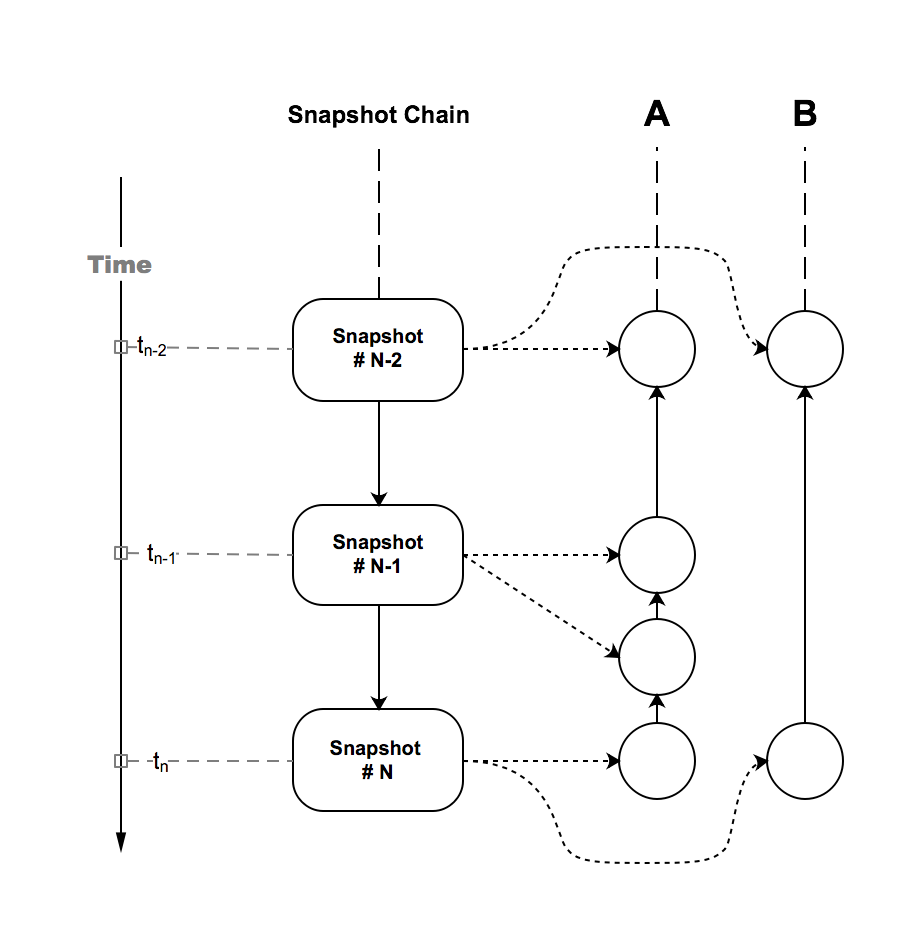
\includegraphics[width=.8\linewidth]{image/snapshotchain-clock.png}
\caption{chaîne d'instantané comme une horloge globale}
\end{figurehere}
\end{center}

Comme indiqué ci-dessus, le compte $A$ a généré 4 transactions à 2 intervalles de temps, tandis que le compte $B$ n'a généré que 2 transactions. Par conséquent, le TPS moyen de $A$ dans cette période est 2 fois celui de $B$. Si c'est juste une transaction de transfert, le TPS moyen du compte quantifié est suffisant. Pour les contrats intelligents, chaque échange a une consommation de ressources différente, il est donc nécessaire d'accumuler du gaz pour chaque transaction afin de calculer la consommation moyenne de ressources pendant une période donnée. La consommation moyenne de ressources des transactions $k$ récentes dans une chaîne de compte avec une hauteur de "n" est la suivante:

\begin{equation}
Cost_{k}(T_n) = \frac{k \cdot \sum_{i=n-k+1}^{n}gas_{i}}{timestamp_{n} - timestamp_{n-k+1} + 1} 
\end{equation}

Parmi eux, pour une transaction $T_n$, $timestamp_n$ est l'horodatage de la transaction, c'est-à-dire la hauteur du bloc d'instantané auquel elle fait référence; $gas_n$ est le carburant consommé pour la transaction.

Lors de la vérification d'une transaction, le nœud déterminera si le quota satisfait à la condition: $Cost(T) \leq Q$, et s'il n'est pas satisfait, la transaction sera rejetée. Dans ce cas, les utilisateurs doivent reconditionner une transaction, augmenter les quotas en payant des frais uniques ou attendre une période de temps pour indiquer un instantané supérieur dans la transaction.

\subsubsection{Bail de quota}

Si un utilisateur possède des actifs  \textit{vite} abondants, mais n'a pas besoin d'utiliser autant de quotas de ressources, il peut choisir de louer son quota à d'autres utilisateurs.

Le système de Vite prend en charge un type de transaction spécial pour transférer le droit d'utiliser un quota de ressources de compte. Dans cette transaction, le nombre de \textit{vite} pouvant être mise en gage, l'adresse d'un cessionnaire et la durée d'un bail peuvent être spécifiés. Une fois la transaction confirmée, le quota de ressources correspondant au montant du token sera inclus dans le compte du cessionnaire. Une fois le délai de location dépassé, le quota sera calculé dans le compte du cédant. L'unité de temps de location est la deuxième. Le système sera converti en différence de hauteur du bloc d'instantanés, de sorte qu'il peut y avoir une déviation.

Le revenu de location peut être obtenu par l'utilisateur. Le système Vite fournit uniquement une transaction de transfert de quota, et le prix et le paiement du crédit-bail peuvent être obtenus grâce à un contrat intelligent tiers.

\subsection{Assurance de biens}
En plus du token natif ViteToken, Vite permet également aux utilisateurs d'émettre leurs token.  L'issue des tokens peut être effectuée via une transaction spéciale, Mint Transaction. L'adresse cible de la transaction mint est 0. Dans le champ \textit{data} de la transaction, les paramètres du token sont spécifiés comme suit:

\begin{verbatim}
Mint: {
    name: "MyToken",
   	totalSupply: 99999999900000000000000000,
   	decimals: 18,
   	owner: "0xa3c1f4...fa",
    symbol: "MYT"
}
\end{verbatim}

Une fois la demande acceptée par le réseau, le \textit{vite} inclus dans la transaction mint sera déduit du compte de l'initiateur comme frais de transaction de la Monnaie. Le système enregistre les informations du nouveau token et lui attribue un \textit{token\_id}. Tous les soldes des token nouvellement générés seront ajoutées à l'adresse \textit{owner}, c'est-à-dire que le compte propriétaire est le compte de genèse du token.

\subsection{Cross Chain Protocol}
Afin de supporter le transfert de valeur croisée des ressources numériques et d'éliminer «l'îlot de valeur», Vite a conçu un protocole VCTP (Vite Cross-Chain Transfer Protocol).

Pour chaque actif nécessitant une transmission croisée sur la chaîne cible, un token qui lui correspond est nécessaire dans le Vite comme le bon du token cible circulant dans le Vite, appelé ToT (Token of Token). Par exemple, si vous voulez transférer le \textit{ether} dans le compte Ethereum vers Vite, vous pouvez émettre un ToT avec un identifiant de \textit{ETH} dans Vite, la quantité initiale de TOT doit être égale à la quantité totale de \textit{ether}.

Pour chaque chaîne cible, il existe un contrat de passerelle sur Vite pour maintenir la relation de mapping entre les transactions Vite et les transactions de chaîne cible. Dans le groupe de consensus où se trouve le contrat, le nœud responsable de la génération de blocs est appelé relais VCTP. Le relais VCTP doit être le nœud Vite et le nœud complet de la chaîne cible en même temps, et suivre les transactions des deux côtés. Sur la chaîne cible, nous devons également déployer un contrat de passerelle Vite.

Avant que le relais VCTP commence à fonctionner, le ToT correspondant dans Vite doit être transféré au contrat de passerelle. Après cela, l'offre de ToT ne peut être contrôlée que par le contrat de passerelle, et personne ne peut être ajouté pour assurer le taux d'échange 1: 1 entre le ToT et l'actif cible. En même temps, les actifs de la chaîne cible sont contrôlés par le contrat de passerelle Vite, et aucun utilisateur ne peut l'utiliser, de manière à garantir que ToT dispose d'une réserve d'acceptation complète.

\begin{center}
\begin{figurehere}
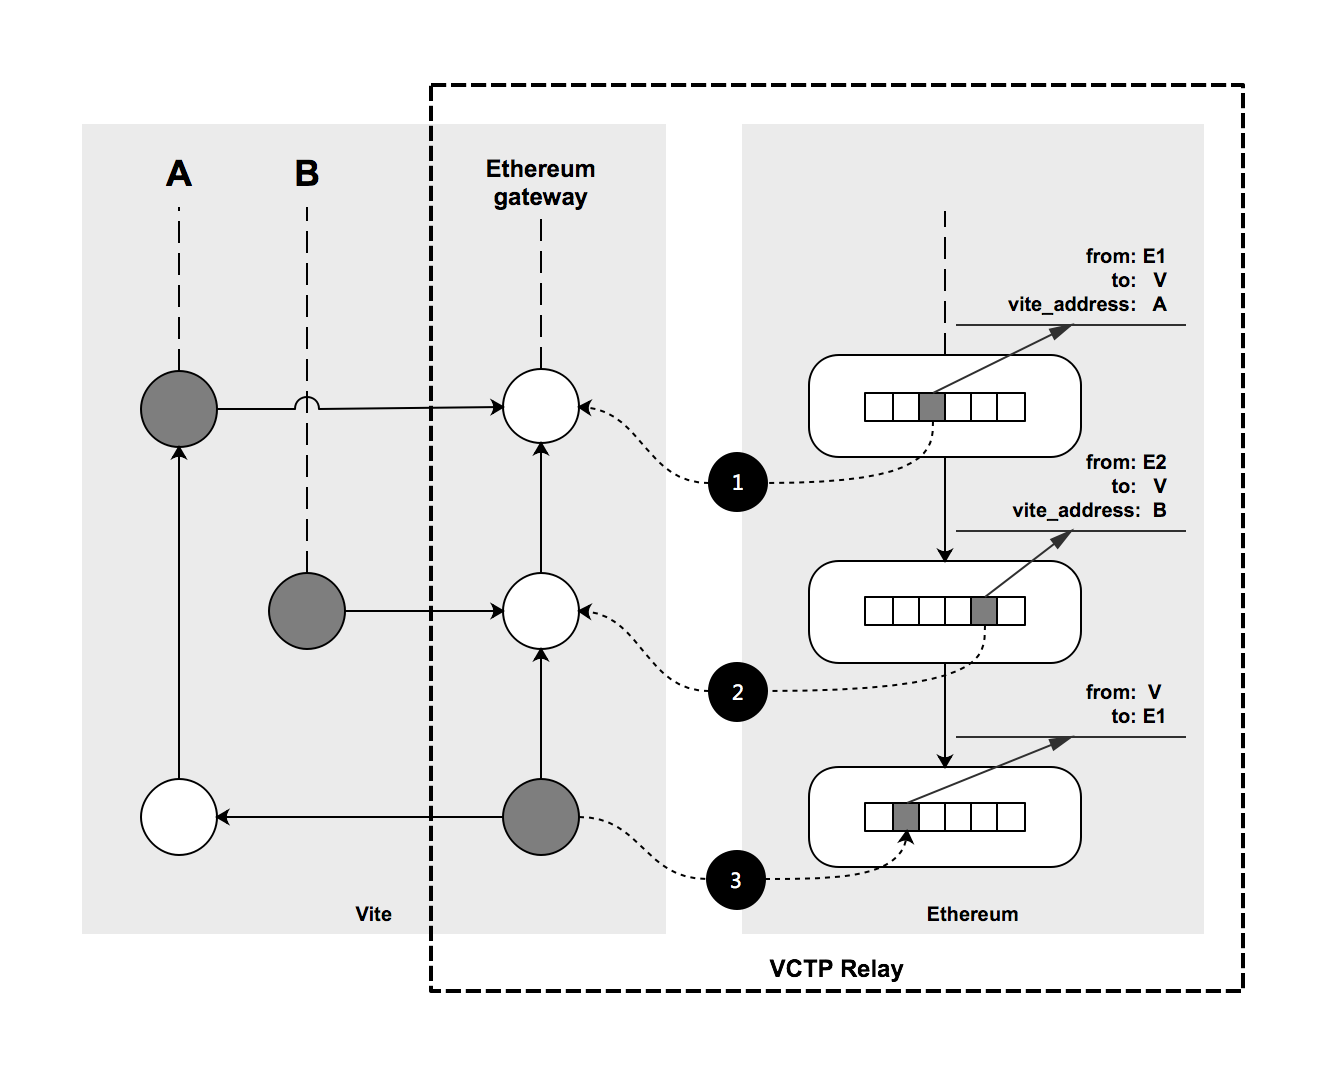
\includegraphics[width=\linewidth]{image/crosschain.png}
\caption{Cross Chain Protocol}
\end{figurehere}
\end{center}

L'image ci-dessus est un exemple de transmission de la valeur de la chaîne croisée entre le Vite et l'Ethereum. Lorsque l'utilisateur Ethereum $E1$ veut transférer le token de l'Ethereum vers le Vite, il peut envoyer une transaction à l'adresse de contrat de passerelle Vite $V$, tandis que l'adresse de l'utilisateur $A$ sur le Vite est placée dans le paramètre. Le solde du transfert sera verrouillé dans le compte de contrat passerelle et deviendra partie de la réserve ToT. Après avoir écouté la transaction, le nœud relais VCTP génère une transaction d'envoi de compte correspondante de Vite, envoyant la même quantité de ToT au compte $A$ de l'utilisateur dans le Vite. Dans l'image, \textcircled{1} et \textcircled{2} indiquent respectivement que $E1$ et $E2$ sont transférés sur le compte Vite $A$ et $B$. Il est à noter que si l'utilisateur ne spécifie pas l'adresse Vite lors du transfert, le contrat rejettera la transaction.

Le flux inverse est indiqué dans \textcircled{3}, Lorsque l'utilisateur $A$ lance le transfert du compte Vite vers le compte Ethereum, une transaction sera envoyée au contrat de passerelle Vite, transférée à une certaine quantité de ToT, et spécifie l'adresse de réception $E1$ de l'Ethereum dans la transaction. Le nœud de relais VCTP va générer le bloc de réponse correspondant sur le contrat "Ethereum Gateway", et empaqueter une transaction de l'Ethereum vers le contrat de passerelle Vite sur l'Ethereum. Dans l'Ethereum, le contrat de passerelle Vite vérifie si cette transaction est initiée par un relais VCTP approuvé, puis la même quantité de \textit{ether} est transférée du contrat de passerelle Vite vers le compte cible $E1$.

Tous les nœuds relais de la chaîne croisée surveillent le réseau cible et peuvent vérifier si chaque transaction inter-chaîne est correcte et parvenir à un consensus au sein du groupe de consensus. Mais le groupe de consensus d'instantanée ne surveillera pas la transaction de la chaîne cible et ne vérifiera pas non plus si le mapping entre les deux chaînes est correct. 
Si le réseau cible est annulé ou durci, les transactions mappées dans le système Vite ne peuvent pas être annulées; De même, si les transactions croisées dans le Vite sont annulées, la transaction correspondante du réseau cible ne peut pas être annulée en même temps. Par conséquent, lorsque vous effectuez des transactions entre chaînes, il est nécessaire de traiter l'annulation de la transaction dans la logique du contrat. En même temps, comme décrit dans la partie \ref{sec:consensus-prio} nous devons définir un paramètre \textit{delay} pour le groupe de consensus relais de la chaîne croisée.

\subsection{Loopring Protocol}
Loopring protocol \ cite {loopring} est un protocole open source pour construire un réseau de trading d'actifs décentralisé. Comparé à d'autres solutions DEX, le protocole Loopring est basé sur le mapping de boucle multipartite, qui fournit une technologie de double autorisation double pour empêcher les transactions préemptives et est entièrement ouverte.

Nous construisons le protocole Loopring dans Vite, ce qui favorise la circulation des actifs numériques dans Vite, de sorte que tout le système de valeurs puisse circuler. Dans ce système de valeurs, les utilisateurs peuvent émettre leurs propres ressources numériques, transférer des ressources en dehors de la chaîne via VCTP et utiliser le protocole Loopring pour réaliser l'échange de ressources. L'ensemble du processus peut être complété dans le système Vite et est complètement décentralisé.

Dans Vite, le protocole de Loopring Smart contract (LPSC) fait partie du système Vite. L'autorisation de transfert d'actifs et la protection atomique multi-parties sont toutes supportés dans Vite. Le relais de Loopring est toujours ouvert à etre intégré pleinement à son propre écosystème.

Les utilisateurs peuvent utiliser \textit{vite} pour payer les transactions d'échange d'actifs, de sorte que le token gagné par les mineurs de Looping qui effectuent le mapping de boucles dans la plate-forme Vite est toujours \textit{vite}.


\section{D'autres conceptions}
\subsection{Planification}
Dans l'Ethereum, les contrats intelligents sont pilotés par des transactions, en plus l'exécution des contrats ne peut être déclenchée que par les utilisateurs initiant une transaction. Dans certaines applications, une fonction d'ordonnancement est nécessaire pour déclencher l'exécution d'un contrat via une horloge.

Dans Ethereum, cette fonction est atteint par des contrats de tiers.\footnote{\textit{Ethereum Alarm Clock} est un contrat tiers utilisé pour planifier l'exécution d'autres contrats, se référer à \url{http://www.ethereum-alarm-clock.com/}}, les performances et la sécurité ne sont pas garanties. Dans Vite, nous ajoutons la fonction d'ordonnancement temporel au contrat intégré. Les utilisateurs peuvent enregistrer leur logique d'ordonnancement dans le contrat d'ordonnancement temporisé. Le groupe de consensus public utilisera la chaîne d'instantanée comme une horloge et enverra la transaction de requête au contrat cible conformément à la logique de planification définie par l'utilisateur.

Il y a un message spécialisé \texttt{Timer} dans Solidity ++. Les utilisateurs peuvent définir leur propre logique de planification dans le code du contrat via \texttt{Timer.on}.

\subsection{Service de nommer}\label{sec:vns}
Dans Ethereum, le contrat va générer une adresse pour identifier un contrat lors de son déploiement. Il y a deux problèmes dans l'identification des contrats avec des adresses:
\begin{itemize}
	\item	Une adresse est un identifiant avec 20 octets sans signification. Il n'est pas aisément utilisable aux utilisateurs et inconvénient à utiliser.
	\item	Les contrats et les adresses ont une un-à-un relation. Ils ne peuvent pas supporter la redirection de contrat.
\end{itemize}

Afin de résoudre ces deux problèmes, le développeur d'Ethereum a fourni un contrat tiers; ENS \footnote{\textit{Ethereum Name Service} est un contrat tiers utilisé pour la résolution de nommer, reportez-vous à \url{https://ens.domains/}}. Cependant, dans le scénario actuel, l'utilisation de services de nommer sera très fréquente, et l'utilisation de contrats tiers ne peut garantir l'unicité globale de la dénomination, nous allons donc construire un service de noms VNS (ViteName Service) dans Vite.

Les utilisateurs peuvent enregistrer un ensemble de noms faciles à retenir et les résoudre à l'adresse réelle via VNS. Les noms sont organisés sous la forme de noms de domaine, tels que\textit{vite.myname.mycontract}. Le nom de domaine de premier niveau sera conservé par le système à des fins spécifiques. Par exemple, \textit{vite.xx} représente l'adresse Vite et \textit{eth.xx} représente une adresse Ethereum. Le nom de domaine de deuxième niveau est open à tous les utilisateurs. Une fois que l'utilisateur possède le nom de domaine de deuxième niveau, le sous-domaine peut être amplifié arbitrairement. Le propriétaire du nom de domaine peut à tout moment modifier l'adresse indiquée par le nom de domaine. Cette fonction peut donc être utilisée pour la mise à niveau du contrat.

La longueur du nom de domaine n'est pas restreinte. Dans VNS, le hash du nom de domaine est réellement stocké. L'adresse cible peut être une adresse non Vite de moins de 256 bits, qui peut être utilisée pour l'interaction entre chaînes.

Nous devons noter que VNS est différent de la spécification du package smart contract EIP190\footnote{\textit{EIP190} Ethereum Smart Contract Packaging Spécification, reportez-vous à \url{https://github.com/ethereum/EIPs/issues/190}} dans Ethereum. VNS est un service de résolution de noms, le nom est établi à l'exécution, et les règles de résolution peuvent être modifiées dynamiquement; 
et EIP190 est une spécification de gestion de package; l'espace de noms est statique et il est établi au moment de la compilation.

\subsection{Mise à jour}
Le contrat intelligent d'Ethereum est immuable. Une fois déployé, il ne peut pas être modifié. Même s'il y a un bug dans le contrat, il ne peut pas être mis à jour. Ceci n'est vraiment pas aisément utilisable aux développeurs et rend l'itération continue de dApp très difficile. Par conséquent, Vite doit fournir un schéma pour prendre en charge la mise à jour des contrats intelligents.

Dans Vite, le processus de mise à jour du contrat comprend:
\begin{itemize}
	\item[A.] Déploie une nouvelle version du contrat pour hériter du statut du contrat d'origine.
	\item[B.] Indique le nom du contrat à la nouvelle adresse dans VNS.
	\item[C.] Supprime l'ancien contrat via l'instruction \textbf{SELFDESTRUCT}.
\end{itemize}

Ces trois étapes doivent être complétées en même temps, et le protocole Vite assure l'atomicité de l'opération. Les développeurs doivent s'assurer que les anciennes données de contrat sont correctement traitées dans le contrat de nouvelle version.

Nous devons noter que le nouveau contrat n'héritera pas de l'adresse de l'ancien contrat. Si cité par l'adresse, la transaction sera toujours envoyée à l'ancien contrat. En effet, différentes versions de contrats sont essentiellement deux contrats totalement différents, qu'ils soient ou non modifiables dynamiquement, en fonction de la sémantique des contrats.

Dans les systèmes Vite, les contrats intelligents sont en fait divisés en deux types, le premier est en fait une circonstance d'un dApp, et sa logique métier est décrite; et la seconde est une sorte de contrat qui cartographie le monde réel. Le précédent est équivalent au service de circonstance d'une application, qui doit être continuellement réitéré lors d'une mise à niveau; ce dernier est équivalent à un contrat, et une fois qu'il entre en vigueur, aucune modification ne peut être faite, sinon c'est une rupture de contrat. Pour un tel contrat qui n'est pas autorisé à être modifié, il peut être décoré avec le mot-clé \textit{static} dans Solidity ++, par exemple:

\begin{verbatim}
pragma solidity++ ^0.1.0;

static contract Pledge {
    // the contract that will never change
}
\end{verbatim}

\subsection{Bloc élagage}
Dans un livre, toute transaction est immuable et les utilisateurs peuvent uniquement ajouter de nouvelles transactions au livre sans modifier ou supprimer les transactions historiques. Par conséquent, avec l'opération du système, les livres deviendront de plus en plus gros. Si un nouveau noeud qui rejoint le réseau veut restaurer le dernier état, en commençant par le bloc de genèse et en refaisant toutes les transactions historiques. Après avoir exécuté le système pendant un certain temps, l'espace occupé par le livre de comptes et le temps nécessaire pour refaire les transactions deviendront inacceptables. Pour le système à haut chargement et déchargement de Vite, le taux de croissance sera beaucoup plus élevé que Bitcoin et Ethereum, il est donc nécessaire de fournir une technique pour écrêter les blocs dans les livres.

BL'écrêtage de bloc fait référence à la suppression des transactions historiques qui ne peuvent pas être utilisées dans les livres, et n'affecte pas l'opération de machine d'état transactionnelle. Alors, quelles transactions peuvent être supprimées en toute sécurité? Cela dépend du scénario dans lequel la transaction sera utilisée, y compris:


\begin{itemize}
\item \textbf{Récupération}.Le rôle principal d'une transaction est de récupérer le statut. Parce que dans Vite, la chaîne d'instantané stocke les informations d'instantané sur l'état du compte, les noeuds peuvent récupérer l'état à partir d'un bloc d'instantané. Toutes les transactions avant \textit{lastTransaction} dans le bloc de capture instantanée peut être adapté à la récupération d'état.
\item \textbf{Vérification des transactions}.Pour vérifier une nouvelle transaction, elle doit vérifier la transaction précédente de l'échange dans la chaîne de compte, et s'il s'agit d'une transaction de réponse, elle doit également vérifier la transaction de demande correspondante. Par conséquent, dans les livres comptables personnalisés, au moins une dernière transaction doit être conservée dans chaque chaîne de compte. En outre, toutes les transactions de demande ouvertes ne peuvent pas être adaptées car leurs hachages peuvent être référencés par des transactions de réponse ultérieures.
\item \textbf{Calculer les quotas.}Si une transaction atteint le quota, elle est calculée en évaluant la moyenne glissante des 10 dernières ressources de transaction, de sorte qu'au moins les 9 dernières transactions doivent être sauvegardées sur chaque chaîne de compte.
\item \textbf{Renseignez-vous sur l'histoire}. Si le noeud a besoin d'interroger l'historique des transactions, la transaction impliquée dans la requête ne sera pas personnalisée.
\end{itemize}

Selon différents scénarios d'usage, chaque nœud peut choisir plusieurs combinaisons a partir de la stratégie de découpage ci-dessus. Il est important de noter que l'écrêtage implique des transactions dans les livres, tandis que les chaînes d'instantanés doivent rester intactes. En outre, ce qui est enregistré dans la chaîne d'instantanés est le hash de l'état du contrat. Lorsque le compte est écrêté, l'état correspondant de l'instantané doit rester intact.

Afin de garantir l'intégrité des données Vite, nous devons conserver certains «nœuds complets» dans le réseau pour enregistrer toutes les données de transaction. Les nœuds de groupe consensus Snapshot sont des nœuds complets, et en outre, des utilisateurs importants tels que des échanges peuvent également devenir des nœuds complets.

\section{Gouvernance}
Pour une plate-forme d'application décentralisée, un système de gouvernance efficace est essentiel pour maintenir un écosystème. L'efficacité et l'équité doivent être prises en compte lors de la conception des systèmes de gouvernance.

Le système de gouvernance de Vite est divisé en deux parties: en-chaine et dehors-chaîne. en-chaine est un mécanisme de vote basé sur le protocole, et dehors-chaîne est l'itération du protocole lui-même.

Sur le mécanisme de vote, il est divisé en deux types: le vote global et le vote local. Le vote global est basé sur le \textit{vite} détenu par l'utilisateur pour calculer les droits comme poids de vote. Le vote global est principalement utilisé pour l'élection du nœud proxy du groupe de consensus d'instantanée. Le vote local vise un contrat. Lorsque le contrat est déployé, un token est désigné comme base pour le vote. Il peut être utilisé pour choisir les nœuds d'agent du groupe de consensus dans lequel se trouve le contrat.

Outre la vérification des transactions, le noeud agent du groupe de consensus d'instantanée a le droit de choisir de mettre à niveau l'Incompatibilité du système Vite. Le noeud proxy du groupe de consensus délégué a le droit de décider s'il faut autoriser la mise à niveau du contrat afin d'éviter les risques potentiels découlant de l'escalade des contrats. Le nœud agent est utilisé pour améliorer le pouvoir de décision au nom des utilisateurs afin d'améliorer l'efficacité de la prise de décision et d'éviter l'échec de la prise de décision en raison d'une participation insuffisante au vote. Ces nœuds proxy eux-mêmes sont également limités par un protocole de consensus. Uniquement si la plupart des \footnote{according to DPoS protocol, the valid majority is 2/3 of total agent nodes.} Les nœuds d'agent sont passés, la mise à niveau prendra effet. Si ces agents ne remplissent pas leur pouvoir de décision en fonction des attentes de l'utilisateur, les utilisateurs peuvent également annuler leur qualification de proxy par voter.

La gouvernance hors-chaîne est réalisée par la communauté. Tout participant de la communauté Vite peut proposer un plan d'amélioration pour le protocole Vite lui-même ou des systèmes connexes, appelé VEP (Vite Enhancement Proposal). VEP peut être largement discuté dans la communauté et si la mise en œuvre de la solution est décidée par les participants écologiques Vite. Si le protocole sera mis à niveau pour la mise en œuvre d'un VEP sera finalement décidé par le nœud de l'agent. Bien sûr, lorsque les différences sont importantes, vous pouvez également commencer un tour de vote sur la chaîne pour recueillir un large éventail d'opinions d'utilisateurs, et le noeud proxy décidera s'il faut mettre à niveau en fonction du résultat du vote.

Bien que certains participants de Vite n'aient pas assez de token \textit{vite} pour voter pour leurs opinions. Mais ils peuvent soumettre librement le VEP et exprimer pleinement leurs avis. Les utilisateurs qui ont le droit de vote doivent prendre pleine responsabilité de la santé de l'ensemble de l'écologie pour leurs propres droits de Vite, et donc ils doivent prendre au sérieux les opinions de tous les participants écologiques.


\section{Tâches à terme}
La vérification des transactions sur les chaînes d'instantané est un goulot d'étranglement majeur sur des performances du système. Parce que Vite adopte une structure asynchrone et une structure de compte DAG, la validation des transactions peut être exécutée en parallèle. Cependant, dû à la dépendance entre les transactions de différents comptes, le degré de parallélisme sera fortement restreint. Comment améliorer le parallélisme de la vérification des transactions ou adopter une stratégie de vérification distribuée sera une sujet importante pour l'optimisation future.

Certaines lacunes existent également dans l'algorithme de consensus HDPoS actuel. C'est aussi une direction de sujet d'optimisation pour améliorer l'algorithme de consensus, ou pour être compatible avec plus d'algorithmes de consensus dans le groupe de consensus délégué.

En outre, l'optimisation de la machine virtuelle est également très importante pour réduire les délais du système et améliorer le chargement et déchargement du système. En raison de la conception simple d'EVM et de la simplification de l'ensemble d'instructions, il peut être nécessaire de concevoir une machine virtuelle plus performante et de définir un langage de programmation de contrat intelligent avec plus de capacité à décrire et moins de failles de sécurité.

Enfin, outre l'accord de noyau de Vite, la construction d'installations auxiliaires qui supporte le développement écologique est également un sujet important. En plus de la prise en charge SDK pour les développeurs dApp, il y a beaucoup de travail à faire dans la construction d'un écosystème de premier plan dApp. Par exemple, vous pouvez créer un moteur dApplet basé sur HTML5 dans l'application de portefeuille mobile de Vite, ce qui permet aux développeurs de développer et de publier dApp avec un coût moins cher.

\section{Sommaire}
Par rapport à d'autres projets similaires, les caractéristiques de Vite comprennent:

\begin{itemize}
	\item \textbf{Haut chargement et déchargement}.Vite utilise la structure du livre DAG, la transaction orthogonale peut être écrite en parallèle au livre; en outre, plusieurs groupes de consensus ne dépendent pas l'un de l'autre dans l'algorithme de consensus HDPoS et peuvent travailler en parallèle; le plus important est que la communication interne de contrat de Vite est basée sur le modèle asynchrone du message. Tout cela est utile pour améliorer le chargement et déchargement du système.
	\item \textbf{Faible retard}.Vite utilise l'algorithme de consensus HDPoS pour collaborer pour terminer le bloc de production de rotation via le noeud proxy, sans avoir besoin de calculer le PoW, l'intervalle de bloc peut être réduit à 1 seconde, ce qui est bénéfique pour réduire le délai de confirmation de transaction.
	\item \textbf{Évolutivité}.Afin de répondre aux exigences d'évolutivité, Vite limite la transaction à un seul degré de liberté, en regroupant les transactions dans le compte en fonction de la dimension du compte, ce qui permet de compléter la production de différents comptes par différents nœuds et de supprimer La sémantique ACID des appels de contrat croisés à la sémantique BASE basée sur le message. De cette façon, les nœuds n'ont plus besoin de sauvegarder tout l'état du monde, et les données sont sauvegardées dans le réseau distribué entier en mode sharding.
	\item \textbf{Utilisabilité}.Les améliorations de l'utilisabilité de Vite comprennent le support de bibliothèque standard dans Solidité++, dédié au traitement de la syntaxe des messages, le calendrier de contrat, les services de nommage VNS, la prise en charge de la mise à niveau des contrats, etc.
	\item \textbf{La circulation des valeurs}.Vite prend en charge l'émission d'actifs numériques, le transfert de valeur de la chaîne croisée, l'échange de token basé sur le protocole Loopring, etc., formant ainsi un système de valeur complet. Du point de vue de l'utilisateur, Vite est un échange décentralisé entièrement fonctionnel.
	\item \textbf{Économie}.Parce que Vite adopte un modèle d'allocation des ressources basé sur les quotas, les utilisateurs légers qui ne négocient pas fréquemment n'ont pas à payer des frais élevés ou des frais de gaz. Les utilisateurs peuvent choisir différentes façons de changer le calcul. Un quota supplémentaire peut également être transféré à d'autres utilisateurs via un contrat de location de quota pour améliorer l'efficacité de l'utilisation des ressources du système.
\end{itemize}
\section{Remerciement}
Sincèrement, nous tenons à remercier nos consultants pour leurs conseils et leur aide à cet article. Nous aimerions particulièrement apprécier la contribution de l'équipe Loopring et de la communauté Loopring à ce projet. 

Remerciement à ZHANG Xuan pour le travail de traduire ce White Paper en version français.

\end{multicols}

\bibliography{vite}
\bibliographystyle{unsrt}


\begin{appendices}

\section{EVM Instruction set\label{app:evm-instruction-set}}
\subsubsection{0s: Stop and algebraic operation instruction set}
\begin{tabu}{l l l l l l} \savetabu{opcodes}
\toprule

\textbf{No.} & \textbf{Words} & \textbf{POP} & \textbf{PUSH} & \textbf{Semantics in EVM} & \textbf{Semantics in Vite}  \vspace{5pt} \\
0x00 & {\small STOP} & 0 & 0 & Stop to Excute. &  Sanme semantics\\
\midrule
0x01 & {\small ADD} & 2 & 1 & Add two operands. & Same semantics\\
\midrule
0x02 & {\small MUL} & 2 & 1 & Multiplying two operands. & Same semantics\\
\midrule
0x03 & {\small SUB} & 2 & 1 & Subtracting two operands. & Same semantics\\
\midrule
0x04 & {\small DIV} & 2 & 1 & Divide two operands & Same semantics\\
&&&&  If the divisor is 0 \\ 
&&&&  then returns 0 \\

\midrule
0x05 & {\small SDIV} & 2 & 1 & Divided with symbol. & Same semantics\\
\midrule
0x06 & {\small MOD} & 2 & 1 & Modulus Operation. & Same semantics\\
\midrule
0x07 & {\small SMOD} & 2 & 1 & Modulus with symbol. & Same semantics\\
\midrule
0x08 & {\small ADDMOD} & 3 & 1 &Add the first two & Same semantics\\
&&&& operands and module with 3rd \\

\midrule
0x09 & {\small MULMOD} & 3 & 1 & Mmultiply the first two  & Same semantics\\
&&&& operands and module with 3rd \\
\midrule
0x0a & {\small EXP} & 2 & 1 & The square of two operands. & Same semantics\\
\midrule
0x0b & {\small SIGNEXTEND} & 2 & 1 & Symbol extension. & Same semantics\\
\midrule
\end{tabu}

\subsubsection{10s: Comparison and bit operation instruction set}
\begin{tabu}{\usetabu{opcodes}}
\toprule
\textbf{No.} & \textbf{Words} & \textbf{POP} & \textbf{PUSH} & \textbf{Semantics in EVM} & \textbf{Semantics in Vite}  \vspace{5pt} \\

0x10 & {\small LT} & 2 & 1 & less than. &  Same semantics\\
\midrule
0x11 & {\small GT} & 2 & 1 & greater than. &  Same semantics\\
\midrule
0x12 & {\small SLT} & 2 & 1 & less than with symbol. &  Same semantics\\
\midrule
0x13 & {\small SGT} & 2 & 1 & greater than with symbol. &  Same semantics\\
\midrule
0x14 & {\small EQ} & 2 & 1 & equal to. &  Same semantics\\
\midrule
0x15 & {\small ISZERO} & 1 & 1 & if it is 0. &  Same semantics\\
\midrule
0x16 & {\small AND} & 2 & 1 & And by bit. &  Same semantics\\
\midrule
0x17 & {\small OR} & 2 & 1 & Or by bit. &  Same semantics\\
\midrule
0x18 & {\small XOR} & 2 & 1 & Xor by bit. &  Same semantics\\
\midrule
0x19 & {\small NOT} & 1 & 1 & Nor by bit. &  Same semantics\\
\midrule
0x1a & {\small BYTE} & 2 & 1 & Take one of byte  &  Same semantics\\
&&&& from the second operands.\\

\bottomrule
\end{tabu}

\subsubsection{20s: SHA3 instruction set}
\begin{tabu}{\usetabu{opcodes}}
\toprule
\textbf{No.} & \textbf{Words} & \textbf{PoP} & \textbf{PUSH} & \textbf{Semantics in EVM} & \textbf{Semantics in Vite} \vspace{5pt} \\
0x20 & {\small SHA3} & 2 & 1 & Calculate Keccak-256 hash. &  Same semantics\\

\bottomrule
\end{tabu}

\subsubsection{30s: Environmental information instruction set}
\begin{tabu}{\usetabu{opcodes}}
\toprule
\textbf{No.} & \textbf{Words} & \textbf{POP} & \textbf{PUSH} & \textbf{Semantics in EVM} & \textbf{Semantics in Vite}  \vspace{5pt} \\

0x30 & {\small ADDRESS} & 0 & 1 & Obtain address . &  Same semantics\\
&&&& of current account \\
\midrule
0x31 & {\small BALANCE} & 1 & 1 &  Obtain the balance &  Same semantics.\\
&&&&  of an account.\\
&&&&& returned is the \\
&&&&&  \textit{vite} balance of account\\
\midrule
0x32 & {\small ORIGIN} & 0 & 1 & Obtain the sender   & Different samantics\\
&&&& addresss of original transaction\\
&&&&& return 0 forever\\
&&&&& Vite doesn't maintain \\
&&&&& the causal relationship \\
&&&&& between internal transaction \\
&&&&& and user transaction.\\
\midrule
0x33 & {\small CALLER} & 0 & 1 & Obtain the address  & Same semantics.\\
&&&& of direct caller.\\
\midrule
0x34 & {\small CALLVALUE} & 0 & 1 & Obtain the transferred  & Same semantics\\
&&&& amount in called transaction.\\
\midrule
0x35 & {\small CALLDATALOAD} & 1 & 1 & Obtain the parameter & Same semantics\\
&&&&  in this calling\\
\midrule
0x36 & {\small CALLDATASIZE} & 0 & 1 & Obtain size of  & Same semantics\\
&&&& parameter \\
&&&& data in this calling.\\
\midrule
0x37 & {\small CALLDATACOPY} & 3 & 0 & Copy called parameter & Same semantics \\
&&&&  data into memory.\\
\midrule
0x38 & {\small CODESIZE} & 0 & 1 & Obtain the size  & Same semantics\\
&&&& of the running code in \\
&&&& current environment.\\
\midrule
0x39 & {\small CODECOPY} & 3 & 0 & Copy the running  & Same semantics\\
&&&& code in current environment \\
&&&& into memory.\\
\midrule
0x3a & {\small GASPRICE} & 0 & 1 & Obtain the gas . & Different samantics\\
&&&& price in current enviroment\\
&&&&& ,return 0 forever.\\
\midrule
0x3b & {\small EXTCODESIZE} & 1 & 1 & Obtain the code  & Same semantics \\
&&&& size of an account.\\
\midrule
0x3c & {\small EXTCODECOPY} & 4 & 0 & Copy the code of. & Same semantics\\
&&&&  an account into memory\\
\midrule
0x3d & {\small RETURNDATASIZE} & 0 & 1 & Obtain data size  & Same semantics\\
&&&& of returned from \\
&&&& previous calling.\\
\midrule
0x3e & {\small RETURNDATACOPY} & 3 & 0 & Copy the returned  &  Same semantics\\
&&&& data calling \\
&&&& previously into memory\\
&&&& into memory.\\
\bottomrule
\end{tabu}

\subsubsection{40s: Block info instructions set}
\begin{tabu}{\usetabu{opcodes}}
\toprule
\textbf{No.} & \textbf{Words} & \textbf{POP} & \textbf{PUSH} & \textbf{Semantics in EVM} & \textbf{Semantics in Vite}  \vspace{5pt} \\

0x40 & {\small BLOCKHASH} & 1 & 1 & Obtain hash of a block. & Different semantic.\\
&&&&& return Hash of  \\
&&&&& corresponing snapshot block.\\
\midrule
0x41 & {\small COINBASE} & 0 & 1 & Obtain the address. & Different semantic.\\
&&&&  of miner beneficiary \\
&&&& in current block\\
&&&&& return 0 forever. \\
\midrule
0x42 & {\small TIMESTAMP} & 0 & 1 & Return timestamp  & Different semantic.\\
&&&& of current block.\\
&&&&& return 0 forever. \\
\midrule
0x43 & {\small NUMBER} & 0 & 1 & Return the number  & Different semantic.\\
&&&& or current block.\\
&&&&& Return the number of \\
&&&&& responding transaction \\
&&&&& block in account chain \\
\midrule
0x44 & {\small DIFFICULTY} & 0 & 1 & Return the difficulty & Different semantic.\\
&&&&  of the block.\\
&&&&& return 0 forever. \\
\midrule
0x45 & {\small GASLIMIT} & 0 & 1 & Return the gas. & Different semantic.\\
&&&&  limitation of the block\\
&&&&& return 0 forever. \\
\bottomrule
\end{tabu}

\subsubsection{50s: Stach, Memory, Storege, Control stream operation instruction set}
\begin{tabu}{\usetabu{opcodes}}
\toprule
\textbf{No.} & \textbf{Words} & \textbf{POP} & \textbf{PUSH} & \textbf{Semantics in EVM} & \textbf{Semantics in Vite}  \vspace{5pt} \\

0x50 & {\small POP} & 1 & 0 & Pop one data & Same semantics\\
&&&&  from top of stack.\\
\midrule
0x51 & {\small MLOAD} & 1 & 1 & load a word from memory. & Same semantics\\

\midrule
0x52 & {\small MSTORE} & 2 & 0 & Save a word to memory & Same semantics\\

\midrule
0x53 & {\small MSTORE8} & 2 & 0 & Save a byte to memory. & Same semantics\\

\midrule
0x54 & {\small SLOAD} & 1 & 1 & Load a word from storage. & Same semantics\\

\midrule
0x55 & {\small SSTORE} & 2 & 0 & Save a word into storage. & Same semantics\\
\midrule
0x56 & {\small JUMP} & 1 & 0 & Jump instructions. & Same semantics\\
\midrule
0x57 & {\small JUMPI} & 2 & 0 & Jump instructions with condition. & Same semantics\\
\midrule
0x58 & {\small PC} & 0 & 1 & Obtain program counter's value. & Same semantics\\
\midrule
0x59 & {\small MSIZE} & 0 & 1 & Obtain size of memory. & Same semantics\\
\midrule
0x5a & {\small GAS} & 0 & 1 & Obtain available gas . &  Different semantic.\\
&&&&& return 0 forever. \\
\midrule
0x5b & {\small JUMPDEST} & 0 & 0 & Mark a destination of jumping . & Same semantics\\
\bottomrule
\end{tabu}

\subsubsection{60s and 70s: Stack operation instructions}
\begin{tabu}{\usetabu{opcodes}}
\toprule
\textbf{No.} & \textbf{Words} & \textbf{POP} & \textbf{PUSH} & \textbf{Semantics in EVM} & \textbf{Semantics in Vite}  \vspace{5pt} \\

0x60 & {\small PUSH1} & 0 & 1 & Push one byte object. & Same semantics\\
&&&&  into top of stack\\

\midrule
0x61 & {\small PUSH2} & 0 & 1 & Push two bytes object  & Same semantics \\
&&&& into top of stack.\\

\midrule
\multicolumn{1}{c}{\vdots} & \multicolumn{1}{c}{\vdots} & \vdots & \vdots & \multicolumn{1}{c}{\vdots} \\
\midrule
0x7f & {\small PUSH32} & 0 & 1 & Push 32 bytes object   & Same semantics \\
&&&& (whole word) into \\
&&&& top of stack\\

\bottomrule
\end{tabu}

\subsubsection{80s: Duplication operation instructions}
\begin{tabu}{\usetabu{opcodes}}
\toprule
\textbf{No.} & \textbf{Words} & \textbf{POP} & \textbf{PUSH} & \textbf{Semantics in EVM} & \textbf{Semantics in Vite}  \vspace{5pt} \\

0x80 & {\small DUP1} & 1 & 2 & Duplicate 1st object and & Same semantics \\
&&&&  push it into top of stack.\\

\midrule
0x81 & {\small DUP2} & 2 & 3 & Duplicate 2nd object  . & Same semantics \\
&&&& and push it into top of stack.\\

\midrule
\multicolumn{1}{c}{\vdots} & \multicolumn{1}{c}{\vdots} & \vdots & \vdots & \multicolumn{1}{c}{\vdots} \\
\midrule
0x8f & {\small DUP16} & 16 & 17 & Duplicate 16th object  & Same semantics \\
&&&&  and push it into top of stack.\\

\bottomrule
\end{tabu}

\subsubsection{90s: Swap operation instructions}
\begin{tabu}{\usetabu{opcodes}}
\toprule
\textbf{No.} & \textbf{Words} & \textbf{POP} & \textbf{PUSH} & \textbf{Semantics in EVM} & \textbf{Semantics in Vite}  \vspace{5pt} \\

0x90 & {\small SWAP1} & 2 & 2 & Swap 1st and 2nd  & Same semantics \\
&&&& object in stack.\\

\midrule
0x91 & {\small SWAP2} & 3 & 3 & Swap 1st and 3rd  & Same semantics \\
&&&& object in stack.\\

\midrule
\multicolumn{1}{c}{\vdots} & \multicolumn{1}{c}{\vdots} & \vdots & \vdots & \multicolumn{1}{c}{\vdots} \\
\midrule
0x9f & {\small SWAP16} & 17 & 17 & Swap 1st and 17th  & Same semantics \\
&&&& object in stack.\\

\bottomrule
\end{tabu}

\subsubsection{a0s: Log operation instructions}
\begin{tabu}{\usetabu{opcodes}}
\toprule
\textbf{No.} & \textbf{Words} & \textbf{POP} & \textbf{PUSH} & \textbf{Semantics in EVM} & \textbf{Semantics in Vite}  \vspace{5pt} \\

0xa0 & {\small LOG0} & 2 & 0 & Extend log record, & Same semantics\\
&&&& no scheme.\\

\midrule
0xa1 & {\small LOG1} & 3 & 0 & Extend log record,. & Same semantics \\
&&&& 1 scheme\\

\midrule
\multicolumn{1}{c}{\vdots} & \multicolumn{1}{c}{\vdots} & \vdots & \vdots & \multicolumn{1}{c}{\vdots} \\
\midrule
0xa4 & {\small LOG4} & 6 & 0 & Extend log record,. & Same semantics\\
&&&& 4 schemes\\ 

\bottomrule
\end{tabu}

\subsubsection{f0s: System operation instructions}
\begin{tabu}{\usetabu{opcodes}}
\toprule
\textbf{No.} & \textbf{Words} & \textbf{POP} & \textbf{PUSH} & \textbf{Semantics in EVM} & \textbf{Semantics in Vite}  \vspace{5pt} \\

0xf0 & {\small CREATE} & 3 & 1 & Create a new contract. & Same semantics \\

\midrule
0xf1 & {\small CALL} & 7 & 1 & Call another contract. & Different semantic. \\
&&&&& indicate sending \\
&&&&& a message to an account\\
&&&&& The returned vale is 0 forever.\\

\midrule
0xf2 & {\small CALLCODE} & 7 & 1 & Call the code of  & Same semantics \\
&&&& another contract\\
&&&& Change the status of account. \\

\midrule
0xf3 & {\small RETURN} & 2 & 0 & Stop execution  & Same semantics \\
&&&& and return value.\\

\midrule
0xf4 & {\small DELEGATECALL} & 6 & 1 & Call the code of  & Same semantics \\
&&&& another contract, change\\
&&&& contract, change current  \\
&&&& account status keep \\
&&&& original transaction info.\\

\midrule
0xfa & {\small STATICCALL} & 6 & 1 & Call another contract, & Different semantic. \\
&&&&  not allow to change status.\\
&&&&& represents to sending\\
&&&&& message to a contract,\\
&&&&& don't change status of \\
&&&&& target contract.\\
&&&&& return 0 forever.needed result \\
&&&&& Sending another message through \\
&&&&& target contract and return. \\

\midrule
0xfd & {\small REVERT} & 2 & 0 & Stop execution and . & Same semantics \\
&&&& recover status and return value \\
&&&&& no semantics of returning left gas.\\

\midrule
0xfe & {\small INVALID} & $\varnothing$ & $\varnothing$ & invalid instructions. & Same semantics \\
\midrule

0xff & {\small SELFDESTRUCT} & 1 & 0 & Stop execution, & Same semantics \\
&&&& set the contract \\
&&&&  as waiting for deleting\\
&&&& return all balance. \\
\bottomrule
\end{tabu}


\end{appendices}
\end{document}
